\documentclass[conference]{IEEEtran}
\IEEEoverridecommandlockouts

\usepackage[T1]{fontenc}
\usepackage{graphicx}
\usepackage{booktabs}
\usepackage{amsmath}
\usepackage{cite}
\usepackage{xcolor}
\usepackage{url}
\usepackage{multirow}
\usepackage{array}
\usepackage[hidelinks]{hyperref}

\graphicspath{{figures/}}
% Every number in the text is a macro generated from the pipeline outputs
% (reports/metrics.json, reports/*.csv) by src/make_report_tables.py.
% AUTO-GENERATED by src/make_report_tables.py - do not edit by hand
\newcommand{\RawRows}{10{,}000}
\newcommand{\AugRows}{10{,}100}
\newcommand{\CleanRows}{10{,}000}
\newcommand{\TrainRows}{8{,}000}
\newcommand{\TestRows}{2{,}000}
\newcommand{\PlacementRate}{42.0}
\newcommand{\NPlaced}{4{,}197}
\newcommand{\NNotPlaced}{5{,}803}
\newcommand{\LabelsInjected}{1500}
\newcommand{\DupAdded}{100}
\newcommand{\DupRemoved}{100}
\newcommand{\LabelsFixed}{1510}
\newcommand{\InvalidNaN}{41}
\newcommand{\CgpaConverted}{9}
\newcommand{\Capped}{25}
\newcommand{\MissingInjectedPerCol}{300}
\newcommand{\MissingTotal}{1541}
\newcommand{\InvalidInjected}{50}
\newcommand{\TypeNoise}{52}
\newcommand{\MinorityShare}{42.0}
\newcommand{\BestModel}{XGBoost}
\newcommand{\SecondModel}{Random Forest}
\newcommand{\BestTestAUC}{0.869}
\newcommand{\BestTestAcc}{0.797}
\newcommand{\BestTestF}{0.750}
\newcommand{\BestTestPrec}{0.777}
\newcommand{\BestTestRec}{0.726}
\newcommand{\BestTestPRAUC}{0.834}
\newcommand{\BestTestMCC}{0.581}
\newcommand{\BestCVAUC}{0.865}
\newcommand{\BestCVAUCsd}{0.005}
\newcommand{\WorstModel}{KNN}
\newcommand{\WorstCVAUC}{0.860}
\newcommand{\CVAUCRange}{0.005}
\newcommand{\StatDiff}{0.0010}
\newcommand{\StatP}{0.328}
\newcommand{\StatPcorr}{0.499}
\newcommand{\McNemarP}{0.118}
\newcommand{\StatSig}{is not}
\newcommand{\FOneThr}{0.37}
\newcommand{\FOneThrTestF}{0.766}
\newcommand{\FOneThrTestRec}{0.819}
\newcommand{\LCGap}{0.019}
\newcommand{\AblCore}{0.8646}
\newcommand{\AblEng}{-0.0008}
\newcommand{\AblExtra}{+0.0185}
\newcommand{\AblNoSim}{-0.0081}
\newcommand{\EngUsed}{were not}
\newcommand{\TopOne}{AptitudeScore}
\newcommand{\TopTwo}{ProgrammingSkills}
\newcommand{\TopThree}{Certifications}
\newcommand{\LeastFeature}{Internships}
\newcommand{\MeanRho}{0.60}
\newcommand{\RankProg}{2}
\newcommand{\RankAtt}{7}
\newcommand{\MaxVIF}{2.20}
\newcommand{\MaxVIFFeature}{ProgrammingSkills}
\newcommand{\OddsTop}{2.06}
\newcommand{\OddsTopFeature}{AptitudeScore}
\newcommand{\XGBName}{XGBoost}
\newcommand{\NIter}{20}
\newcommand{\CorrInternProg}{0.49}


\begin{document}

\title{Predicting Campus Placement Outcomes of Engineering Students Using Machine Learning and Explainable Feature Analysis}

\author{
\IEEEauthorblockN{[Member 1 Name]}
\IEEEauthorblockA{\textit{[Department]} \\
\textit{[College]}\\
[City], India \\
[email]}
\and
\IEEEauthorblockN{[Member 2 Name]}
\IEEEauthorblockA{\textit{[Department]} \\
\textit{[College]}\\
[City], India \\
[email]}
}

\maketitle

% ===========================================================================
\begin{abstract}
Campus placement is a key outcome for engineering colleges, and early identification of students who are
unlikely to be placed allows the training and placement cell to intervene in time. This paper predicts whether
a student will be placed from eight attributes: CGPA, programming skills, internships, certifications,
communication skills, aptitude score, projects and attendance. A public dataset of \RawRows{} student records is
extended with two documented simulated attributes and with deliberately injected data-quality problems, and is
then processed by a reproducible cleaning and modelling pipeline. Five classifiers---logistic regression,
$k$-nearest neighbours, a support vector machine, random forest and \XGBName{}---are tuned with stratified
5-fold cross-validation. \BestModel{} obtains the highest cross-validated ROC-AUC (\BestCVAUC{}) and reaches a
test ROC-AUC of \BestTestAUC{} and an accuracy of \BestTestAcc{}; the difference to the runner-up \StatSig{}
statistically significant. Feature influence is measured with five independent methods (logistic-regression
coefficients, impurity and gain importance, permutation importance and SHAP) and combined into a consensus
ranking, in which \TopOne{}, \TopTwo{} and \TopThree{} are the most influential attributes. The final model is
deployed in an interactive web application that explains each prediction and suggests the most effective
improvements for an individual student.
\end{abstract}

\begin{IEEEkeywords}
campus placement prediction, educational data mining, machine learning, explainable AI, SHAP, XGBoost
\end{IEEEkeywords}

% ===========================================================================
\section{Introduction}
Placement statistics strongly influence how students, parents and accreditation bodies perceive an engineering
college. Training and placement cells therefore invest considerable effort in aptitude training, mock interviews
and skill development. These resources are limited, so it is valuable to know \emph{which} students are at
risk of not being placed and \emph{which} attributes matter most, early enough for targeted intervention.

Machine learning (ML) classifiers can estimate the probability of placement from academic and skill-related
attributes. A probability alone, however, is of little use to a placement officer unless it is accompanied by
an explanation and by concrete, actionable advice. This work combines predictive modelling with a multi-method
analysis of feature influence.

\textbf{Objectives.}
\begin{itemize}
  \item Build a clean, reproducible pipeline from raw data to a deployable model.
  \item Train and compare at least four classifiers (five are used) under a common, leakage-free protocol.
  \item Identify the most influential features with several independent methods and test whether they agree.
  \item Provide an interactive application for single-student and batch prediction, explanation and what-if advice.
\end{itemize}

\textbf{Contributions.} (i) A fully scripted pipeline in which every reported number is regenerated from data
by a single command; (ii) a fair comparison of five model families with a statistical significance test;
(iii) a consensus ranking of feature influence from five methods, including an ablation that quantifies the
effect of the simulated attributes; and (iv) a deployed web application with per-student explanations.

The rest of the paper is organised as follows. Section~\ref{sec:lit} reviews related work.
Sections~\ref{sec:data}, \ref{sec:prep} and \ref{sec:fe} describe the data, preprocessing and feature
engineering. Sections~\ref{sec:design}, \ref{sec:impl} and \ref{sec:models} cover the design, implementation and
models. Section~\ref{sec:results} presents the results, and Section~\ref{sec:conclusion} concludes.

% ===========================================================================
\section{Literature Survey}\label{sec:lit}
Pathak \emph{et al.}~\cite{pathak2025framework} predict on-campus placement for engineering students using a
public Kaggle dataset of 2{,}966 records with age, gender, stream, internships, CGPA, hostel and history of
backlogs. They compare logistic regression, decision tree, KNN, Gaussian naive Bayes, random forest and
XGBoost, and propose a soft-voting ensemble of KNN, decision tree and random forest tuned with grid search and
10-fold cross-validation. The ensemble reaches an accuracy of 89.23\% and an AUC of 0.943. The authors note that
the dataset is limited to engineering students, which restricts generalisability.

Kumar \emph{et al.}~\cite{kumar2023predicting} predict college placements from academic performance indicators
such as grades, test scores and extracurricular activities. Logistic regression, Gaussian naive Bayes, random
forest, SVM and KNN are compared using accuracy, precision, recall and F1-score, and random forest is reported
as the most effective method. The dataset size and numeric results are not stated in the abstract.

Casuat \emph{et al.}~\cite{casuat2020steps} develop StEPS, an employability prediction system for 1{,}000
engineering students who completed on-the-job training. Principal component analysis is used to identify the
most predictive attributes---communication skills, growth potential and the student performance rating---and
logistic regression performs the prediction. The work relies on a single linear model and on
institution-specific assessment data.

Basha \emph{et al.}~\cite{basha2023unraveling} combine exploratory analysis of academic and demographic
attributes (gender, academic performance, degree and MBA specialisation) with predictive models including
logistic regression and SVM. They conclude that core academic achievement remains a strong influence on
placement, and suggest temporal analysis of placement trends as future work.

Beyond these four studies, Sibagariang~\cite{sibagariang2025interpretable} applies SHAP to job-placement
prediction from graduates' course grades, GPA and internship duration, comparing tree ensembles with logistic
regression, and Mezhoudi \emph{et al.}~\cite{mezhoudi2023employability} survey employability-prediction
approaches and highlight data availability and interpretability as open challenges.

Table~\ref{tab:lit} summarises the surveyed studies. Recurring limitations are (a) evaluation of one model family or reliance on accuracy alone, (b) feature
importance taken from a single method, and (c) small or institution-specific datasets. The present work addresses these gaps by comparing five model families under one
protocol with a significance test, by triangulating feature influence across five methods, and by deploying the
model in an explainable application.

\begin{table*}[t]
\centering
\caption{Comparison of related work on placement and employability prediction}
\label{tab:lit}
\footnotesize
\begin{tabular}{p{2.3cm}p{3.6cm}p{3.6cm}p{2.9cm}p{3.6cm}}
\toprule
Paper & Dataset & Methods & Best reported result & Gap \\
\midrule
Pathak \emph{et al.}~\cite{pathak2025framework} (2025) & Kaggle, 2{,}966 engineering students & LR, DT, KNN, GNB, RF, XGBoost, soft-voting ensemble & Ensemble: accuracy 89.23\%, AUC 0.943 & Single domain; generalisability limited \\
Kumar \emph{et al.}~\cite{kumar2023predicting} (2023) & College students' academic records & LR, GNB, RF, SVM, KNN & RF best (accuracy, precision, recall, F1) & Dataset size and numeric results not given in abstract \\
Casuat \emph{et al.}~\cite{casuat2020steps} (2020) & 1{,}000 engineering OJT students & PCA + logistic regression & Communication skills among top predictors & Single linear model; institution-specific data \\
Basha \emph{et al.}~\cite{basha2023unraveling} (2023) & Academic and demographic attributes & EDA, LR, SVM & High accuracy reported & Dataset size not stated; temporal trends left for future work \\
Sibagariang~\cite{sibagariang2025interpretable} (2025) & Graduates' grades, GPA, internships & DT, RF, XGBoost, LightGBM, CatBoost, LR + SHAP & LR: accuracy 92\% & SHAP only; one explanation method \\
\midrule
This work & \RawRows{} students, 8 core attributes & LR, KNN, SVM, RF, \XGBName{} + 5 importance methods & \BestModel{}: test ROC-AUC \BestTestAUC{} & Two attributes simulated (Section~\ref{sec:data}) \\
\bottomrule
\end{tabular}
\end{table*}

% ===========================================================================
\section{Dataset Description}\label{sec:data}
\subsection{Source}
The base data is the publicly available \emph{Placement Prediction Dataset} (\texttt{placementdata.csv}),
obtained through a Hugging Face mirror~\cite{dataset_hf}. It contains \RawRows{} students with CGPA,
internships, projects, workshops/certifications, aptitude test score, soft-skills rating, extracurricular
activities, placement training, SSC and HSC marks, and the placement status. The mirror stores the rows as
train/validation/test files without a student identifier; they were concatenated and a sequential identifier
was added. The dataset is likely to be at least partly synthetic, which is discussed as a limitation.

\subsection{Simulated attributes}
No public dataset contains all eight attributes of the problem statement. \texttt{ProgrammingSkills} and
\texttt{Attendance} were therefore \textbf{simulated} with a fixed random seed and the following documented
rules, where $z(\cdot)$ is the standardised column and $p\in\{0,1\}$ the original label:
\begin{align*}
\text{Prog} &= \mathrm{clip}\big(\mathrm{round}(5.5 + 1.1z(\text{Proj}) + 0.7z(\text{Intern})\\
            &\quad + 0.4z(\text{CGPA}) + 0.6p + \mathcal{N}(0,1.6^2)),\,1,10\big)\\
\text{Att}  &= \mathrm{clip}\big(80 + 3z(\text{CGPA}) + 2p + \mathcal{N}(0,7.5^2),\,45,100\big)
\end{align*}
The effects were chosen to be modest and were not tuned. Because both rules use the label, any influence
attributed to these two columns reflects the simulation assumptions rather than real-world evidence.

\subsection{Injected data-quality problems}
The public file is already clean. To evaluate a realistic cleaning pipeline, a seeded and logged set of problems
was injected: \MissingInjectedPerCol{} missing values (3\%) in each of five columns, \DupAdded{} exact
duplicate rows, \InvalidInjected{} invalid entries (CGPA above 10 or typed as a percentage, attendance above 100
or negative, aptitude above 100), \LabelsInjected{} inconsistently spelled labels (e.g.\ \texttt{NP},
\texttt{not placed}), inconsistent Yes/No values and numeric values stored as padded strings. The augmented file
has \AugRows{} rows.

\subsection{Attributes and class balance}
Table~\ref{tab:attr} lists the attributes after cleaning. The data contains \NPlaced{} placed and
\NNotPlaced{} not-placed students, a placement rate of \PlacementRate\% (Fig.~\ref{fig:eda}a).
Fig.~\ref{fig:eda}b shows the correlation structure and Fig.~\ref{fig:bins} the placement rate by binned
attribute value: placement rates rise steeply with aptitude score and CGPA, and from one to three projects (the small
group with no recorded projects is an exception).

\begin{table}[t]
\centering
\caption{Attributes after cleaning (summary statistics from the pipeline)}
\label{tab:attr}
\scriptsize
\setlength{\tabcolsep}{3pt}
\begin{tabular}{lllllrl}
\toprule
Attribute & Type & Valid & Observed & Mean $\pm$ SD & Miss.\% & Source \\
\midrule
CGPA & float & 0--10 & 6.5--9.1 & 7.70 $\pm$ 0.64 & 3.1 & Real \\
ProgrammingSkills & int & 1--10 & 1.0--10.0 & 5.72 $\pm$ 2.38 & 3.0 & Simulated \\
Internships & int & 0--3 & 0.0--2.0 & 1.05 $\pm$ 0.67 & 0.0 & Real \\
Certifications & int & 0--5 & 0.0--3.0 & 1.01 $\pm$ 0.90 & 0.0 & Real \\
CommunicationSkills & float & 1--5 & 3.0--4.8 & 4.32 $\pm$ 0.41 & 3.0 & Real \\
AptitudeScore & int & 0--100 & 60.0--90.0 & 79.49 $\pm$ 8.15 & 3.1 & Real \\
Projects & int & 0--5 & 0.0--3.0 & 2.03 $\pm$ 0.87 & 0.0 & Real \\
Attendance & float (\%) & 0--100 & 58.2--100.0 & 80.96 $\pm$ 8.20 & 3.2 & Simulated \\
ExtracurricularActivities & binary & 0/1 & 0--1 & 0.59 $\pm$ 0.49 & 0.0 & Real (ablation) \\
PlacementTraining & binary & 0/1 & 0--1 & 0.73 $\pm$ 0.44 & 0.0 & Real (ablation) \\
SSC\_Marks & int & 0--100 & 55--90 & 69.16 $\pm$ 10.43 & 0.0 & Real (ablation) \\
HSC\_Marks & int & 0--100 & 57--88 & 74.50 $\pm$ 8.92 & 0.0 & Real (ablation) \\
\bottomrule
\end{tabular}

\end{table}

\begin{figure}[t]
\centering
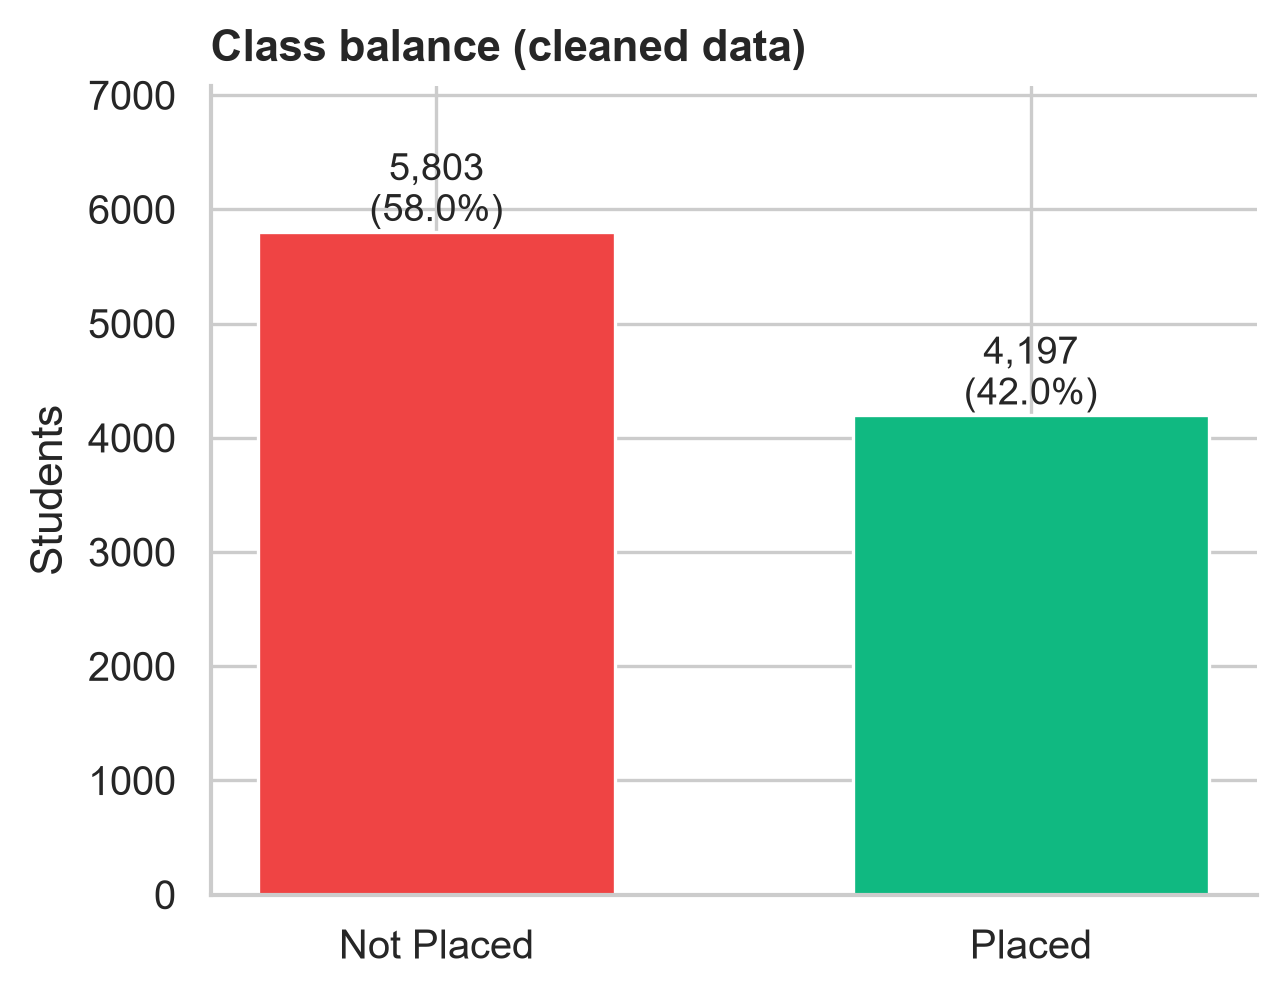
\includegraphics[width=0.48\columnwidth]{class_balance.png}\hfill
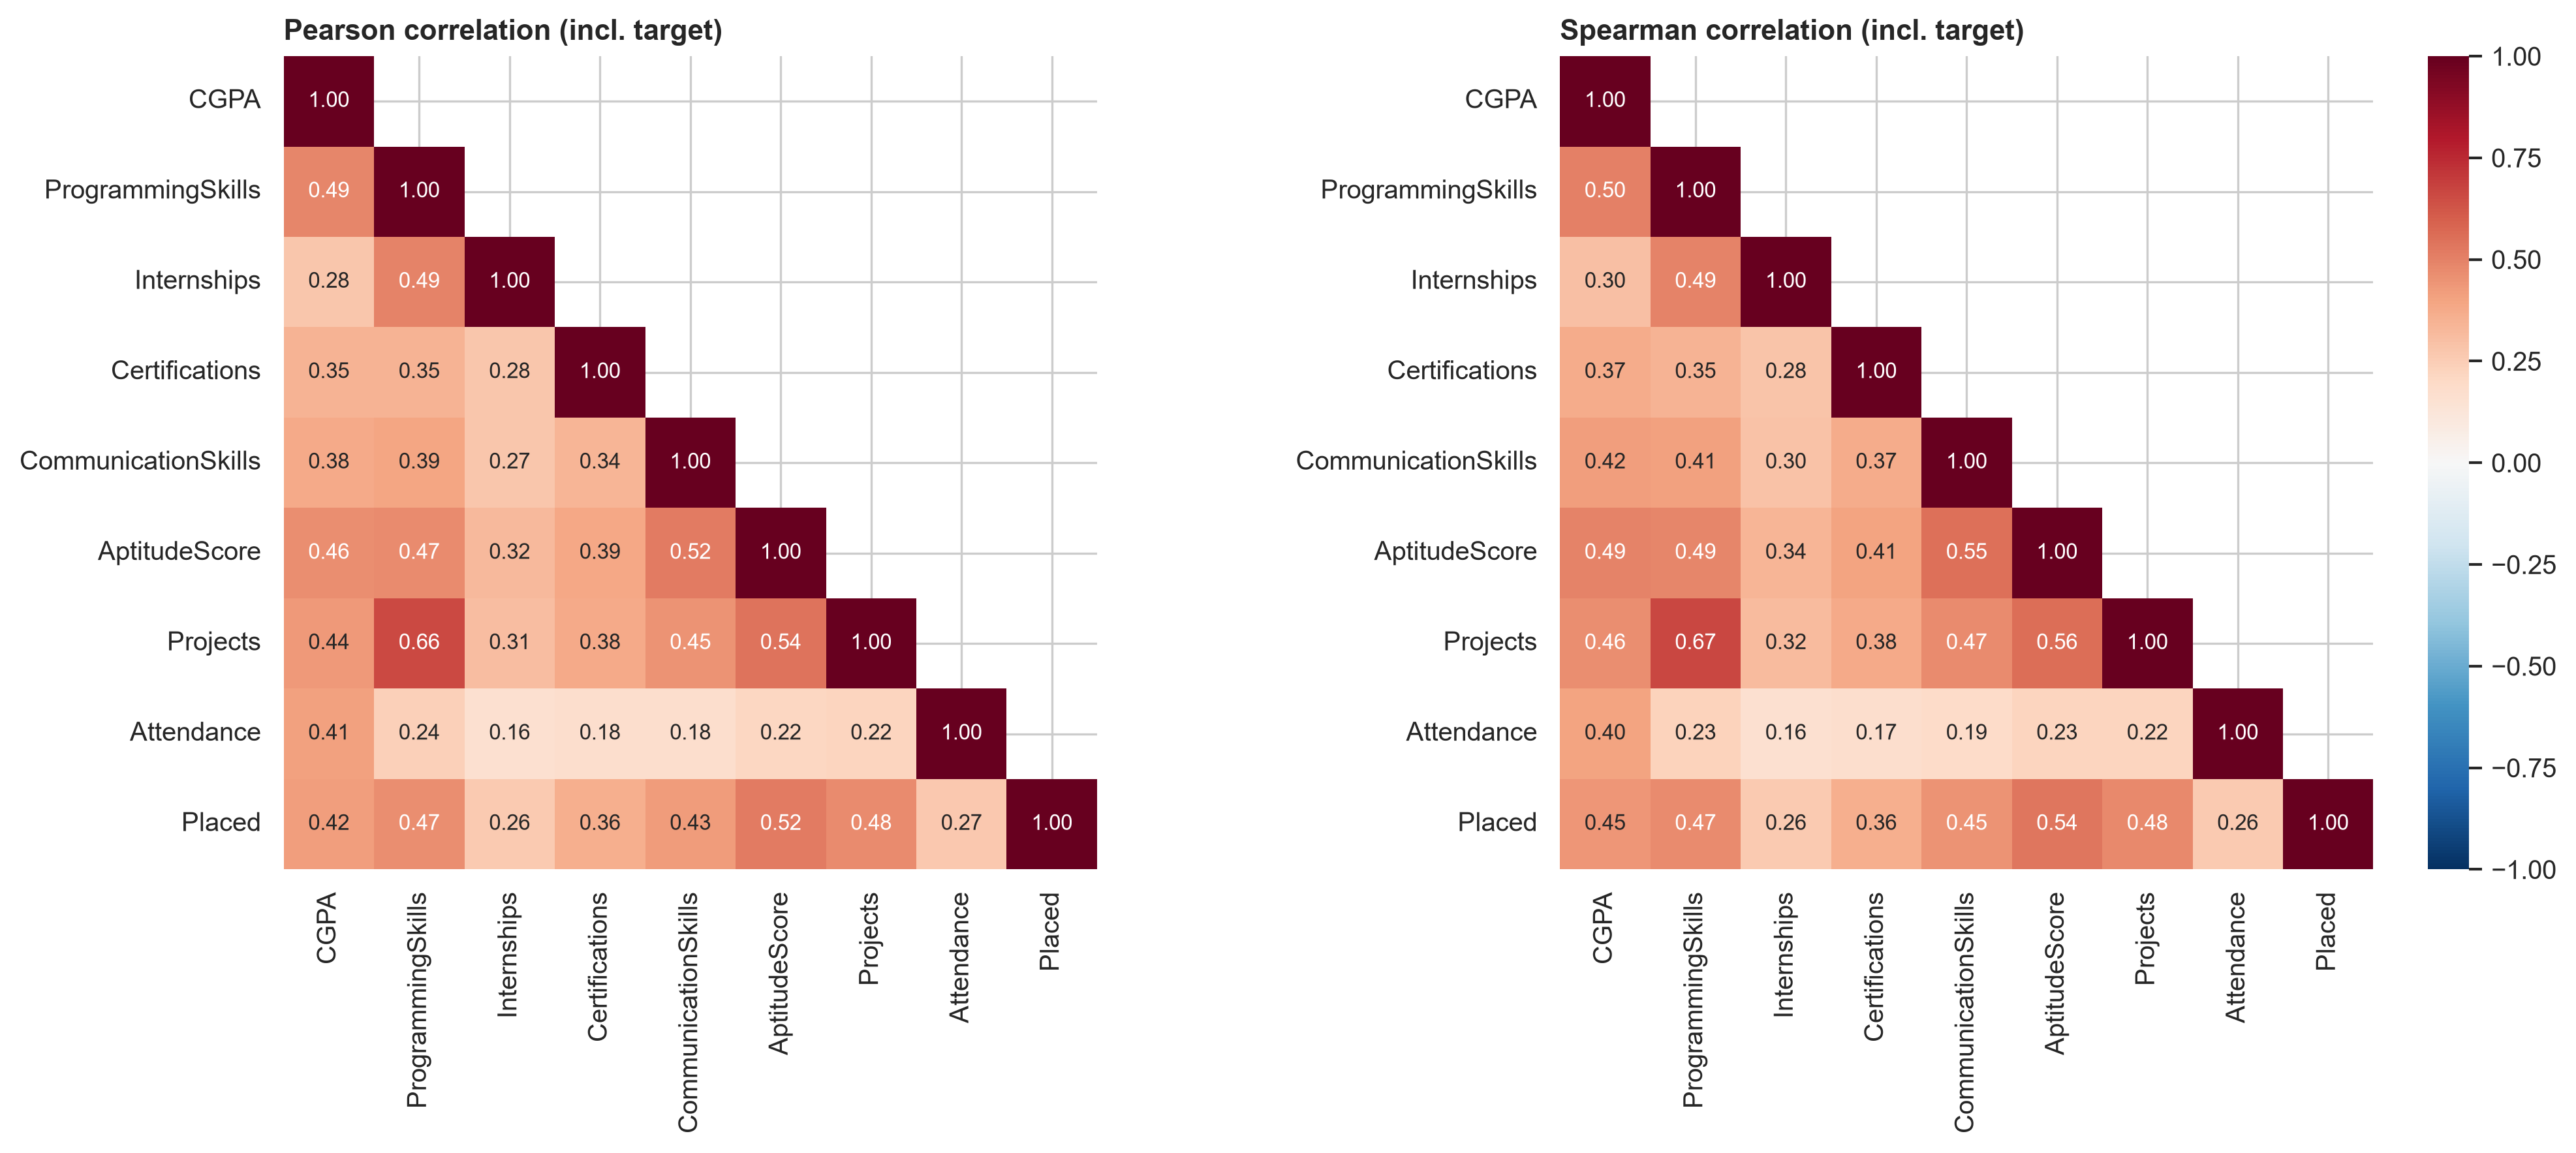
\includegraphics[width=0.50\columnwidth]{correlation_heatmap.png}
\caption{(a) Class balance after cleaning; (b) Pearson and Spearman correlations including the target.}
\label{fig:eda}
\end{figure}

\begin{figure*}[t]
\centering
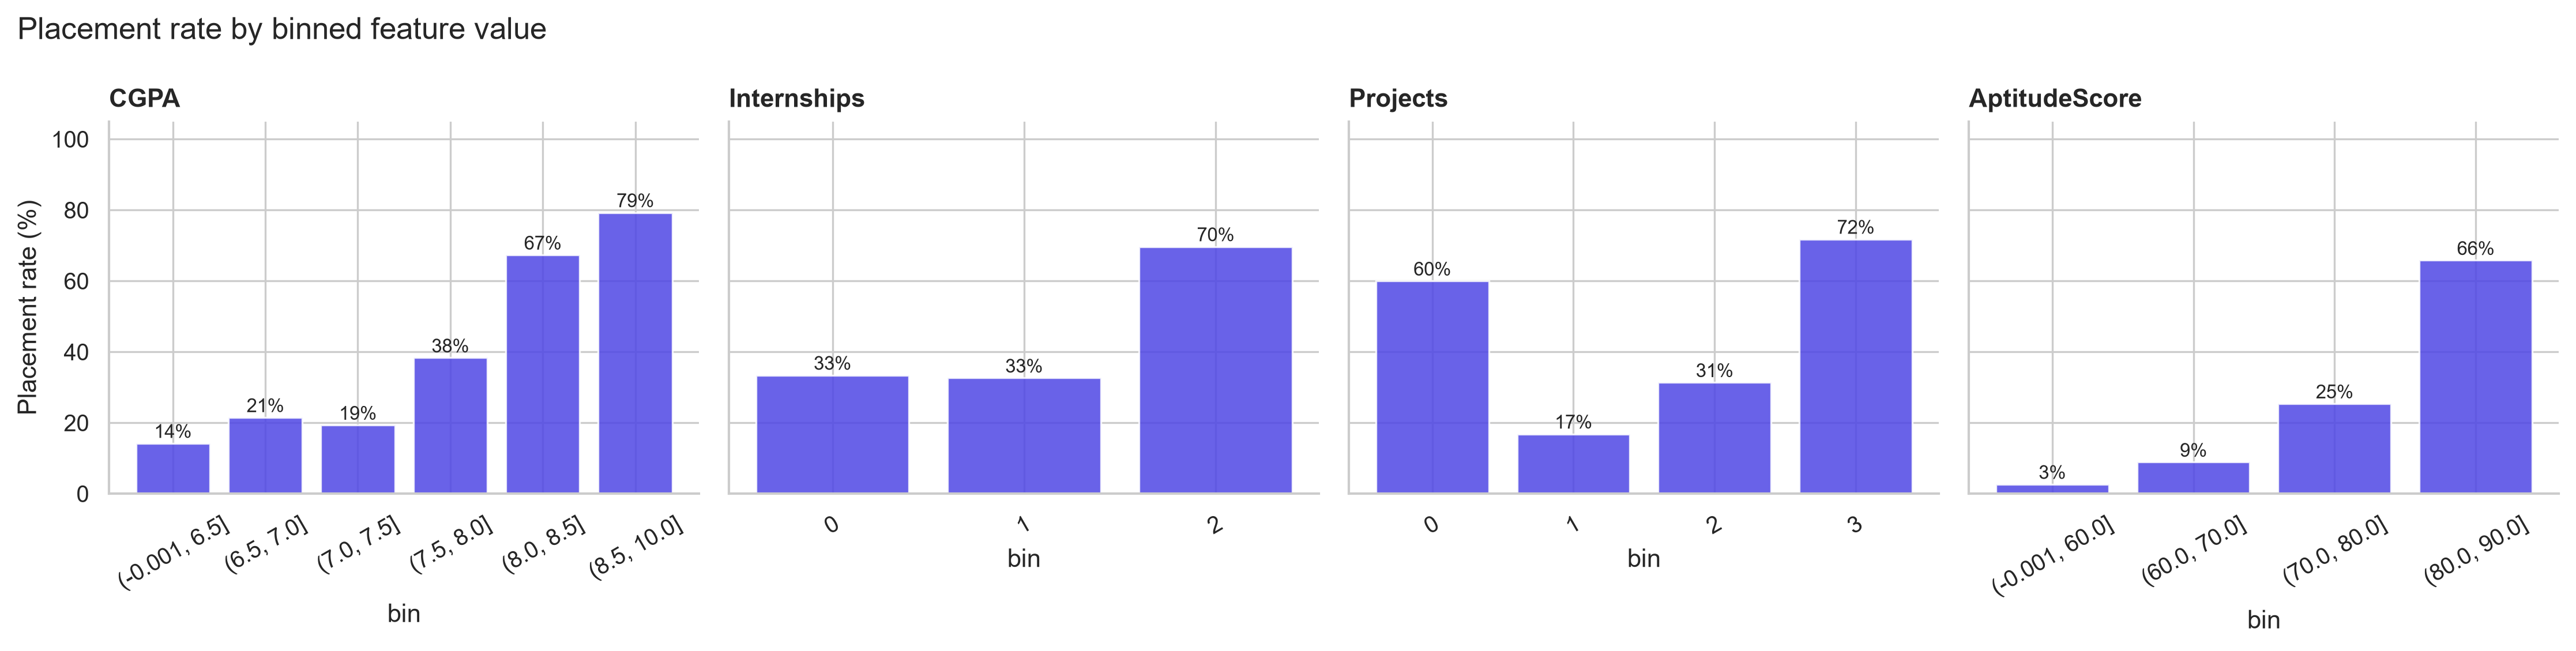
\includegraphics[width=0.9\textwidth]{placement_rate_by_bins.png}
\caption{Placement rate by binned CGPA, internships, projects and aptitude score.}
\label{fig:bins}
\end{figure*}

% ===========================================================================
\section{Data Preprocessing}\label{sec:prep}
Cleaning is implemented in \texttt{src/preprocess.py}; every step logs its counts
(Table~\ref{tab:prep}). The steps, in order, are:
\begin{enumerate}
  \item \emph{Column standardisation} to the final attribute names.
  \item \emph{Whitespace and type coercion}: padded numeric strings are stripped and converted
        (\TypeNoise{} cells).
  \item \emph{Label and categorical normalisation}: all spellings of the target are mapped to 0/1
        (\LabelsFixed{} labels) and Yes/No variants to 1/0.
  \item \emph{Duplicate removal}: \DupRemoved{} exact duplicates are removed. The student identifier is part of
        the comparison so that different students with identical marks are never merged.
  \item \emph{Invalid ranges}: values outside the domain range become missing (\InvalidNaN{} cells). A CGPA
        between 35 and 100 is interpreted as a percentage and converted with $\text{CGPA}=\text{value}/9.5$
        (\CgpaConverted{} cells).
  \item \emph{Stratified split}: 80/20 train/test split (\TrainRows{}/\TestRows{} rows), performed
        \emph{before} any statistic is learned.
  \item \emph{Outlier capping}: continuous attributes are winsorised at $1.5\times$IQR with bounds learned on the
        training rows only (\Capped{} values).
\end{enumerate}
The fixed counts are slightly higher than the injected counts because the duplicated rows also carried injected
problems. The remaining \MissingTotal{} missing cells (injected gaps plus invalid values) are filled by median
imputation \emph{inside} the scikit-learn pipeline. The imputer is therefore fitted on the training folds only
during cross-validation, so no information from validation or test rows leaks into training.
Fig.~\ref{fig:outliers} shows the effect on CGPA, attendance and aptitude score.

\begin{table}[t]
\centering
\caption{Data-quality problems injected and fixed}
\label{tab:prep}
\footnotesize
\setlength{\tabcolsep}{3pt}
\begin{tabular}{lrr}
\toprule
Step & Injected & Fixed / result \\
\midrule
Rows in augmented file & -- & 10100 \\
Whitespace/type noise fixed & 50 & 52 \\
Target labels normalised & 1500 & 1510 \\
Yes/No categoricals normalised & 2000 & 2019 \\
Exact duplicates removed & 100 & 100 \\
CGPA percentage $\rightarrow$ CGPA & 9 & 9 \\
Out-of-range values $\rightarrow$ NaN & 41 & 41 \\
Outliers capped (IQR, 1.5$\times$) & -- & 25 \\
Missing cells imputed (median, in pipeline) & 1500 & 1541 \\
Rows after cleaning & -- & 10000 \\
Train / test rows (stratified 80/20) & -- & 8000 / 2000 \\
\bottomrule
\end{tabular}

\end{table}

\begin{figure}[t]
\centering
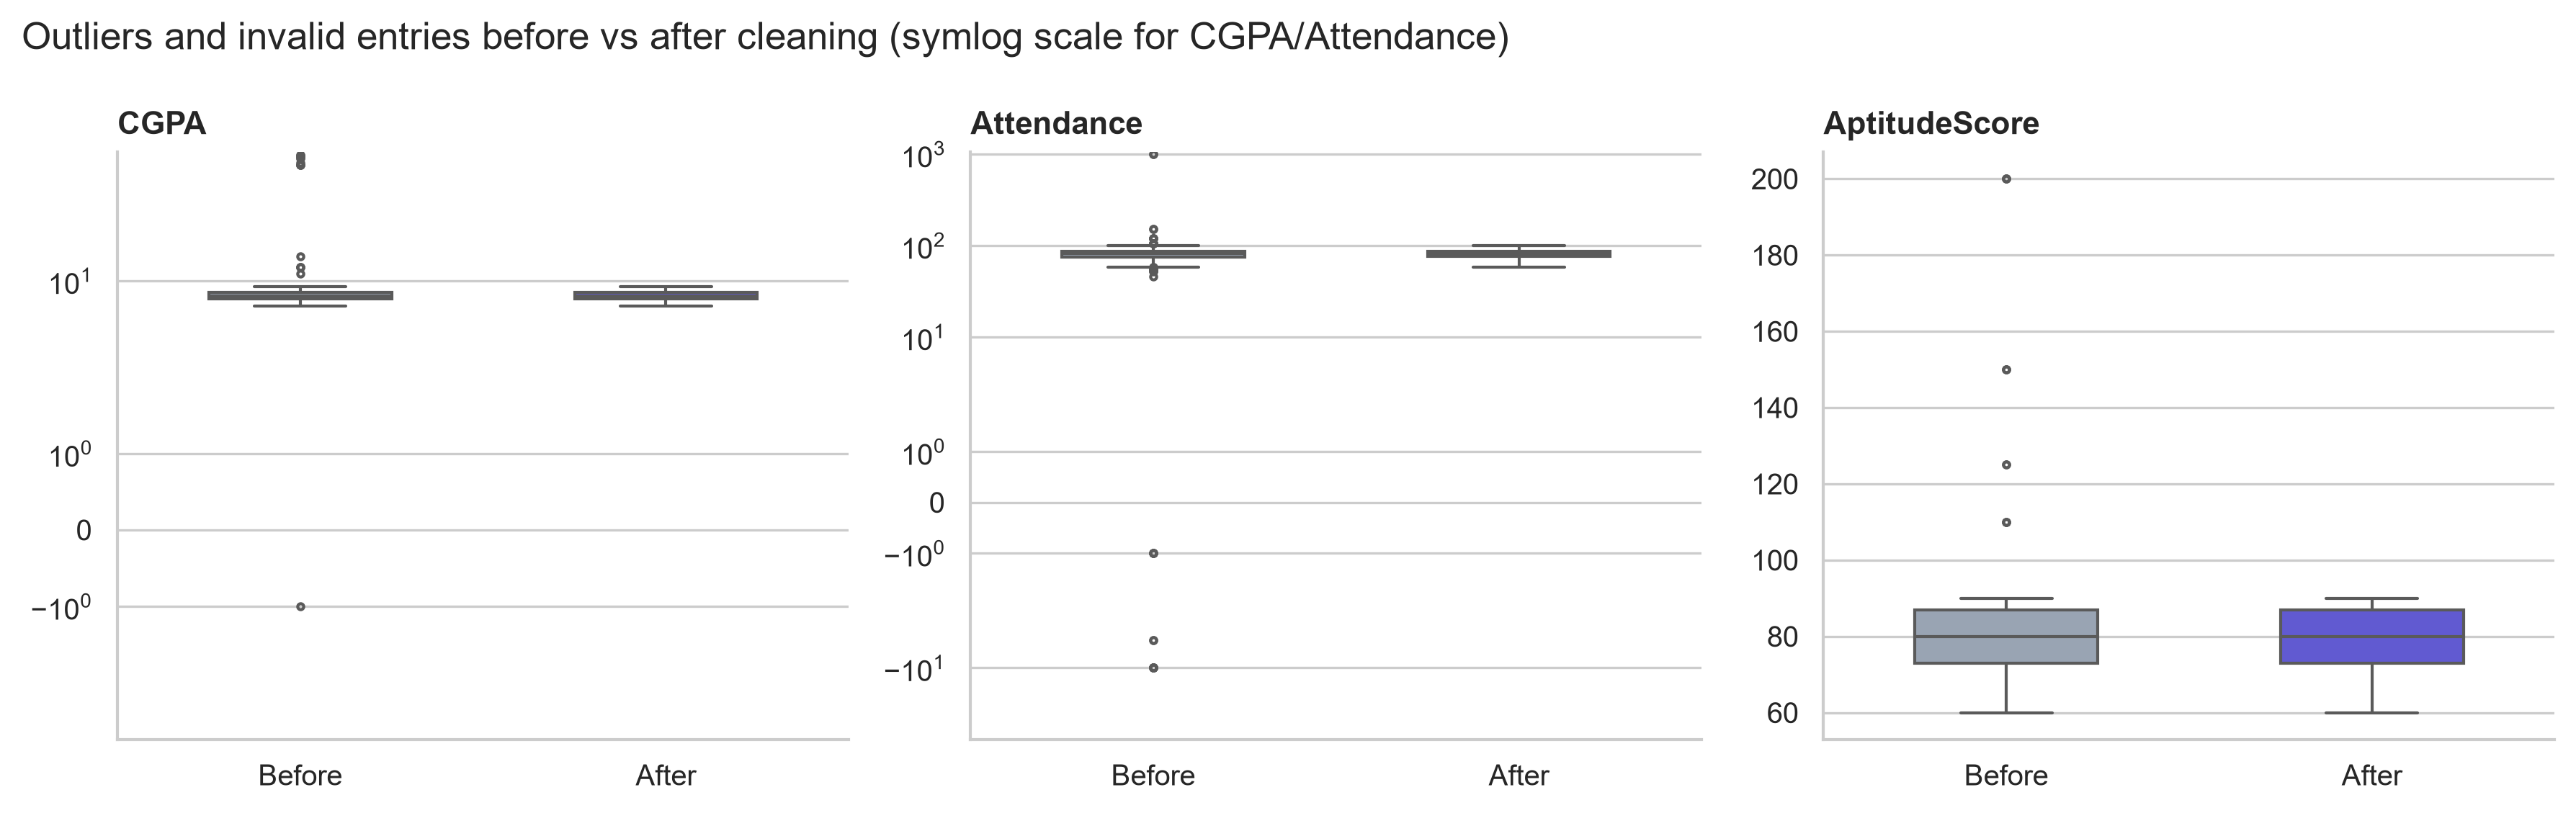
\includegraphics[width=\columnwidth]{outliers_before_after.png}
\caption{Distributions before and after cleaning (symmetric-log scale for CGPA and attendance).}
\label{fig:outliers}
\end{figure}

% ===========================================================================
\section{Feature Engineering}\label{sec:fe}
\subsection{Engineered features}
Three features were constructed: $\text{ExperienceScore}=\text{Internships}+\text{Projects}+\text{Certifications}$,
$\text{SkillIndex}$ as the mean of the standardised programming, communication and aptitude scores, and
$\text{AcademicConsistency}=\text{CGPA}\cdot\text{Attendance}/100$. They are implemented as a scikit-learn
transformer whose standardisation statistics are learned on training data only.

\subsection{Scaling and encoding}
Logistic regression, SVM and KNN depend on distances or gradient magnitudes and receive standardised inputs;
tree ensembles use the unscaled values. The two binary categoricals are already 0/1, so no one-hot encoding is
required.

\subsection{Feature selection and multicollinearity}
Mutual information, the ANOVA $F$-test, the $\chi^2$ test and recursive feature elimination (RFE) with logistic
regression were computed on the training set (Table~\ref{tab:fs}, Fig.~\ref{fig:fs}). All filter methods place
aptitude score at or near the top. The largest variance inflation factor is \MaxVIF{} (\MaxVIFFeature{}), well
below the usual threshold of 5, so multicollinearity is not a concern.

\begin{table}[t]
\centering
\caption{Feature-selection scores (rank in brackets) and VIF}
\label{tab:fs}
\footnotesize
\setlength{\tabcolsep}{3pt}
\begin{tabular}{lrrrrr}
\toprule
Feature & MI (rank) & ANOVA F (rank) & $\chi^2$ (rank) & RFE & VIF \\
\midrule
AptitudeScore & 0.160 (1) & 2842 (1) & 230.2 (2) & 1 & 1.75 \\
Projects & 0.119 (2) & 2252 (2) & 218.2 (3) & 7 & 2.09 \\
ProgrammingSkills & 0.117 (3) & 2125 (3) & 216.9 (4) & 2 & 2.20 \\
CommunicationSkills & 0.111 (4) & 1732 (4) & 98.5 (7) & 3 & 1.49 \\
Certifications & 0.109 (5) & 1264 (6) & 294.0 (1) & 5 & 1.31 \\
CGPA & 0.104 (6) & 1649 (5) & 173.7 (5) & 6 & 1.60 \\
Internships & 0.051 (7) & 621 (7) & 123.5 (6) & 8 & 1.37 \\
Attendance & 0.033 (8) & 610 (8) & 39.0 (8) & 4 & 1.19 \\
\bottomrule
\end{tabular}

\end{table}

\begin{figure*}[t]
\centering
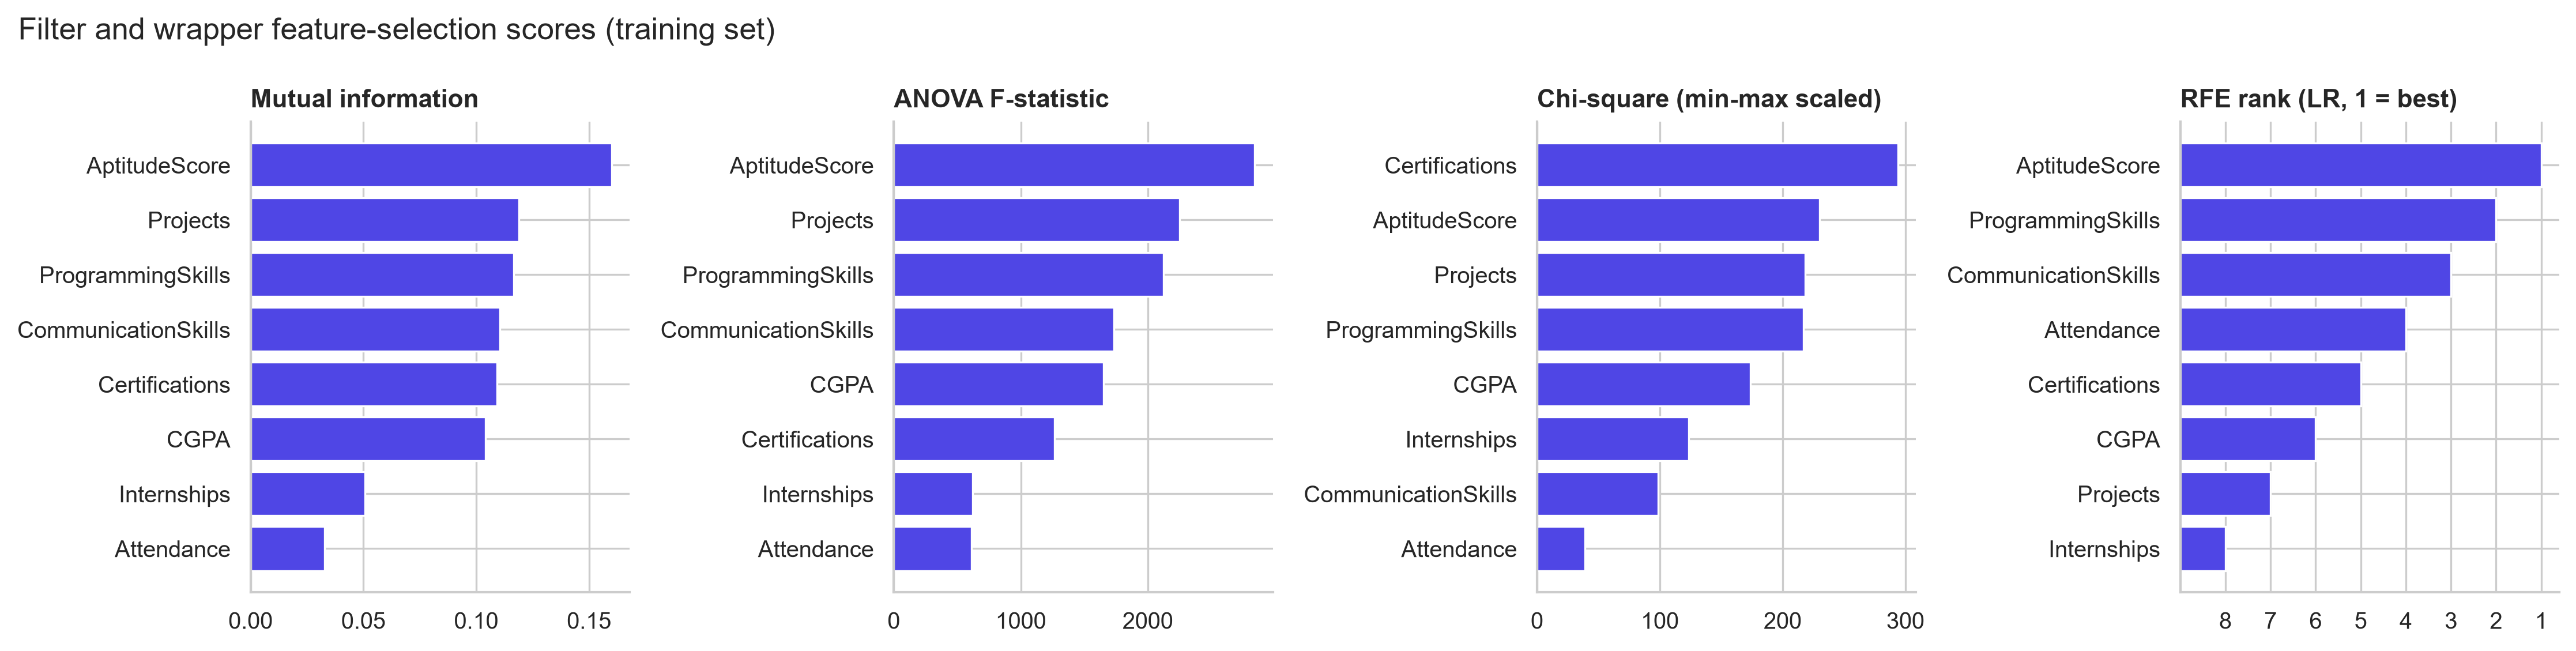
\includegraphics[width=0.95\textwidth]{feature_selection.png}
\caption{Filter (MI, ANOVA, $\chi^2$) and wrapper (RFE) feature-selection results on the training set.}
\label{fig:fs}
\end{figure*}

\subsection{Final feature set}
An ablation study (Section~\ref{sec:ablation}) showed that the engineered features change the cross-validated
ROC-AUC of the best model by \AblEng{}. Since the pre-registered rule required a gain of at least 0.005, the
engineered features \EngUsed{} used, and the final model uses the eight core attributes.

% ===========================================================================
\section{Design Phase}\label{sec:design}
Fig.~\ref{fig:arch} shows the system architecture. The workflow is: (1) download the raw data;
(2) add the simulated attributes and inject quality problems; (3) clean the data and log every fix;
(4) split into stratified training and test sets; (5) analyse and engineer features; (6) tune five model
pipelines with randomised search and 5-fold cross-validation on the training set; (7) select the model with the
highest mean CV ROC-AUC and evaluate it once on the test set; (8) explain the model with five importance methods
and partial dependence; (9) save the full pipeline with its metadata; and (10) serve it in a web application
for single and batch prediction with what-if analysis. A single script (\texttt{run\_all.py}) executes steps
1--9 and regenerates every figure and table in this paper.

\begin{figure*}[t]
\centering
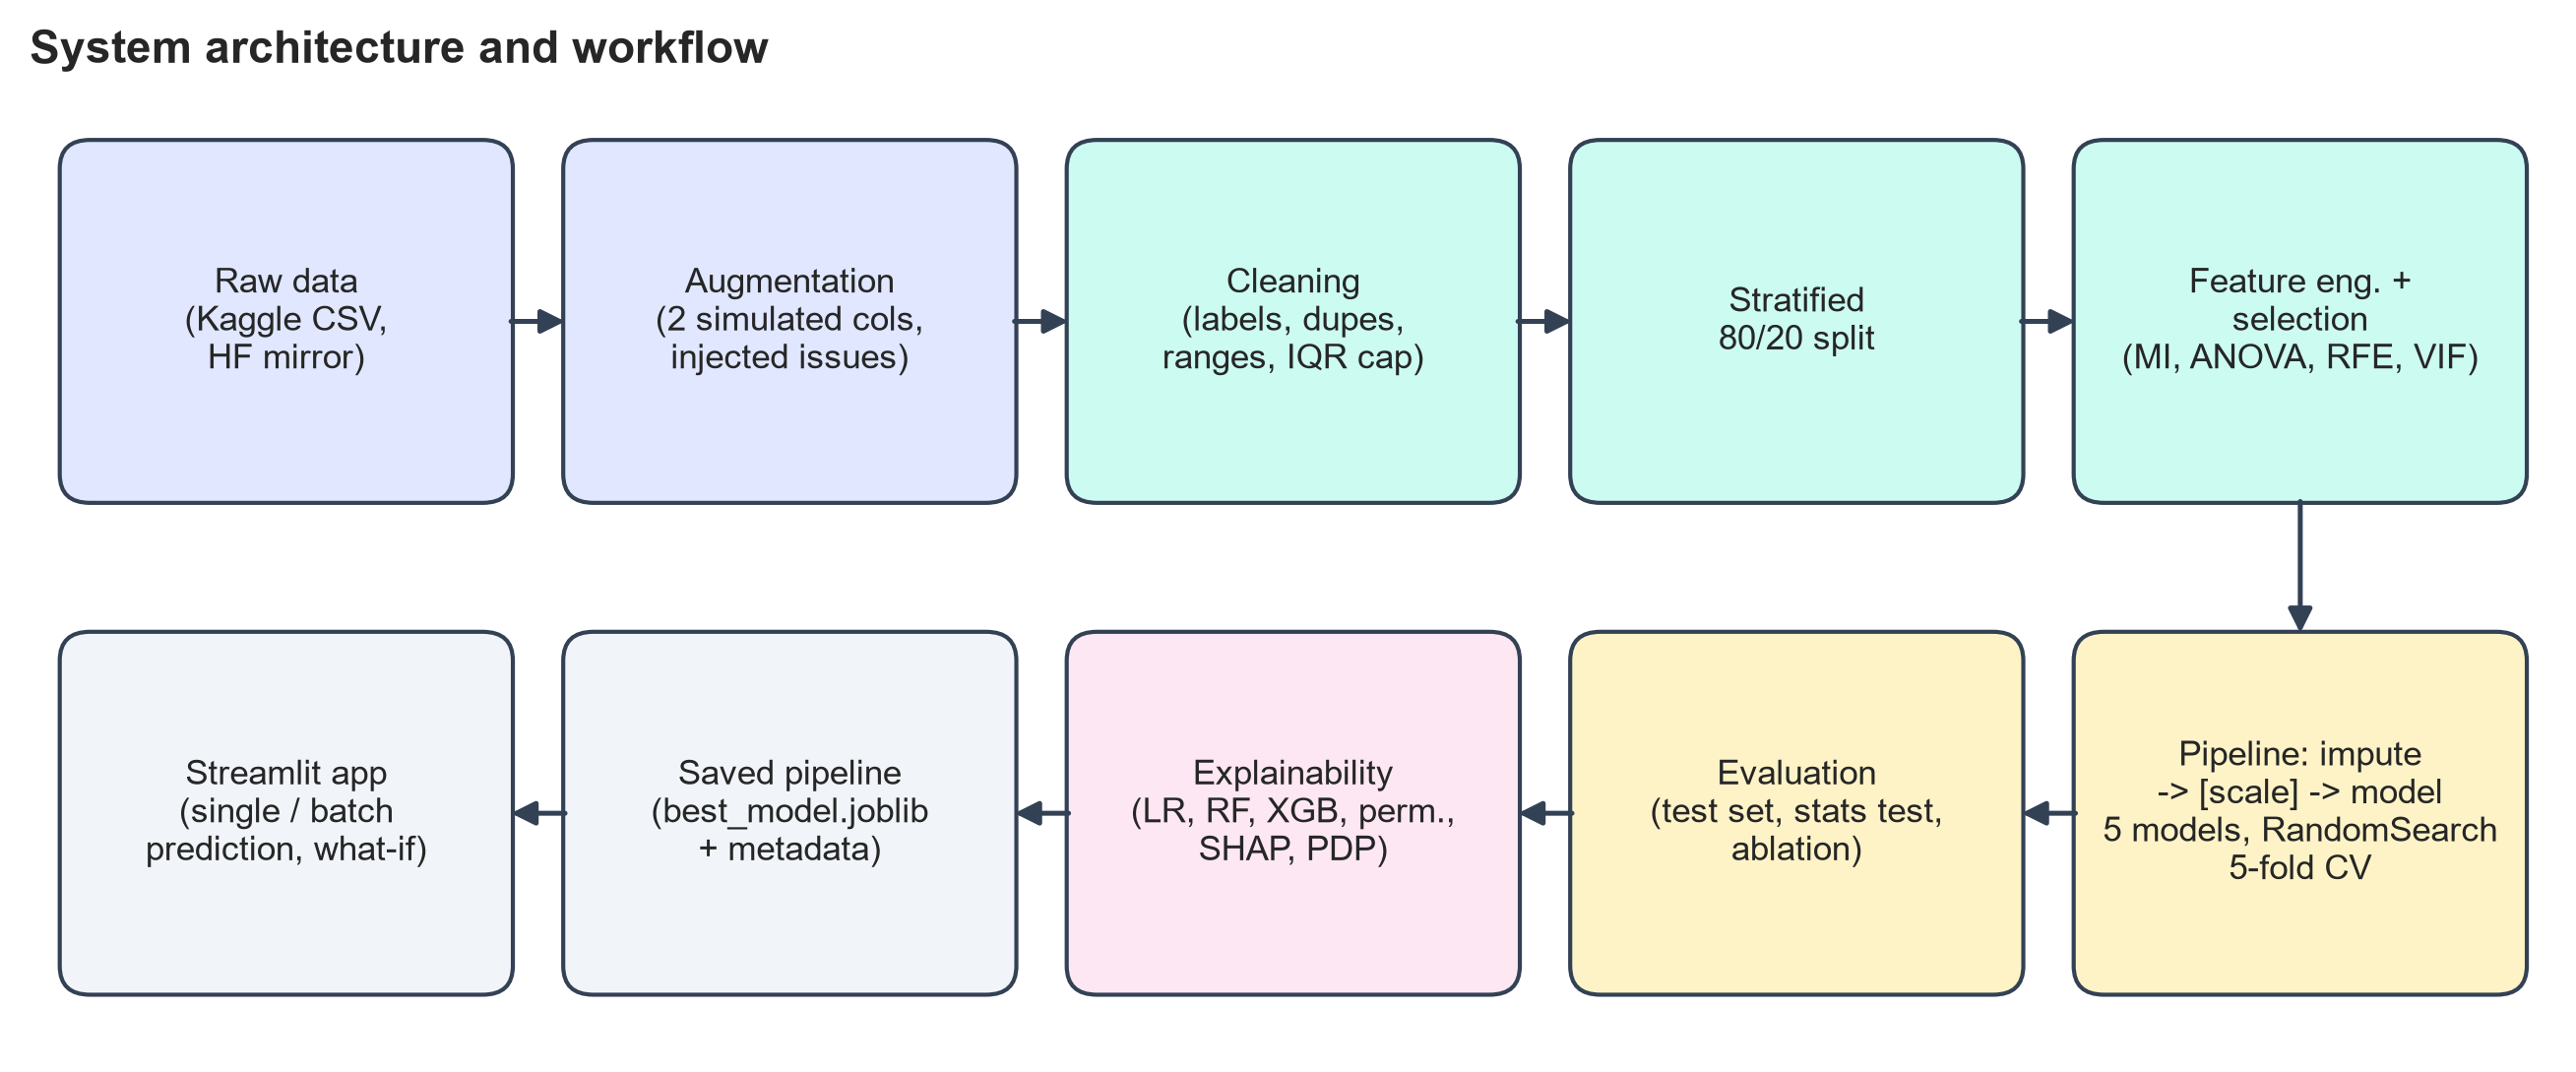
\includegraphics[width=0.9\textwidth]{architecture.png}
\caption{System architecture and workflow.}
\label{fig:arch}
\end{figure*}

% ===========================================================================
\section{Implementation}\label{sec:impl}
The system is implemented in Python with the libraries in Table~\ref{tab:env}. All experiments ran on a laptop
CPU; no GPU is required for tabular models of this size, and the complete pipeline finishes in a few minutes.

\textbf{Experimental setup.} Stratified 80/20 train/test split; stratified 5-fold cross-validation with the same
folds for every model; \texttt{RandomizedSearchCV} with \NIter{} candidates per model (10 for the SVM) and
ROC-AUC as the scoring metric; random seed 42 for every random process. The minority class (placed) forms
\MinorityShare\% of the training set, so no resampling was applied (SMOTE~\cite{chawla2002smote} would be an
alternative for stronger imbalance). The decision threshold is 0.5; the F1-optimal threshold estimated from
out-of-fold predictions is \FOneThr{}, which raises test recall to \FOneThrTestRec{} at an F1 of \FOneThrTestF{}.

\begin{table}[t]
\centering
\caption{Software environment}
\label{tab:env}
\footnotesize
\setlength{\tabcolsep}{3pt}
\begin{tabular}{llll}
\toprule
Library & Version & Library & Version \\
\midrule
Python & 3.12.4 & scipy & 1.18.1 \\
numpy & 2.5.4 & statsmodels & 0.15.0 \\
pandas & 2.3.3 & matplotlib & 3.11.2 \\
scikit-learn & 1.7.2 & seaborn & 0.13.2 \\
xgboost & 3.4.1 & plotly & 6.9.0 \\
shap & 0.54.1 & streamlit & 1.67.0 \\
\bottomrule
\end{tabular}

\end{table}

\textbf{Web application.} A Streamlit application (Fig.~\ref{fig:app}) loads the saved pipeline and offers:
single-student prediction with a probability gauge, a per-student SHAP explanation and the three most effective
single-step improvements; data and feature-influence dashboards; model comparison; and batch scoring of a
CSV file with validation of every row and risk bands for the placement cell.

\begin{figure}[t]
\centering
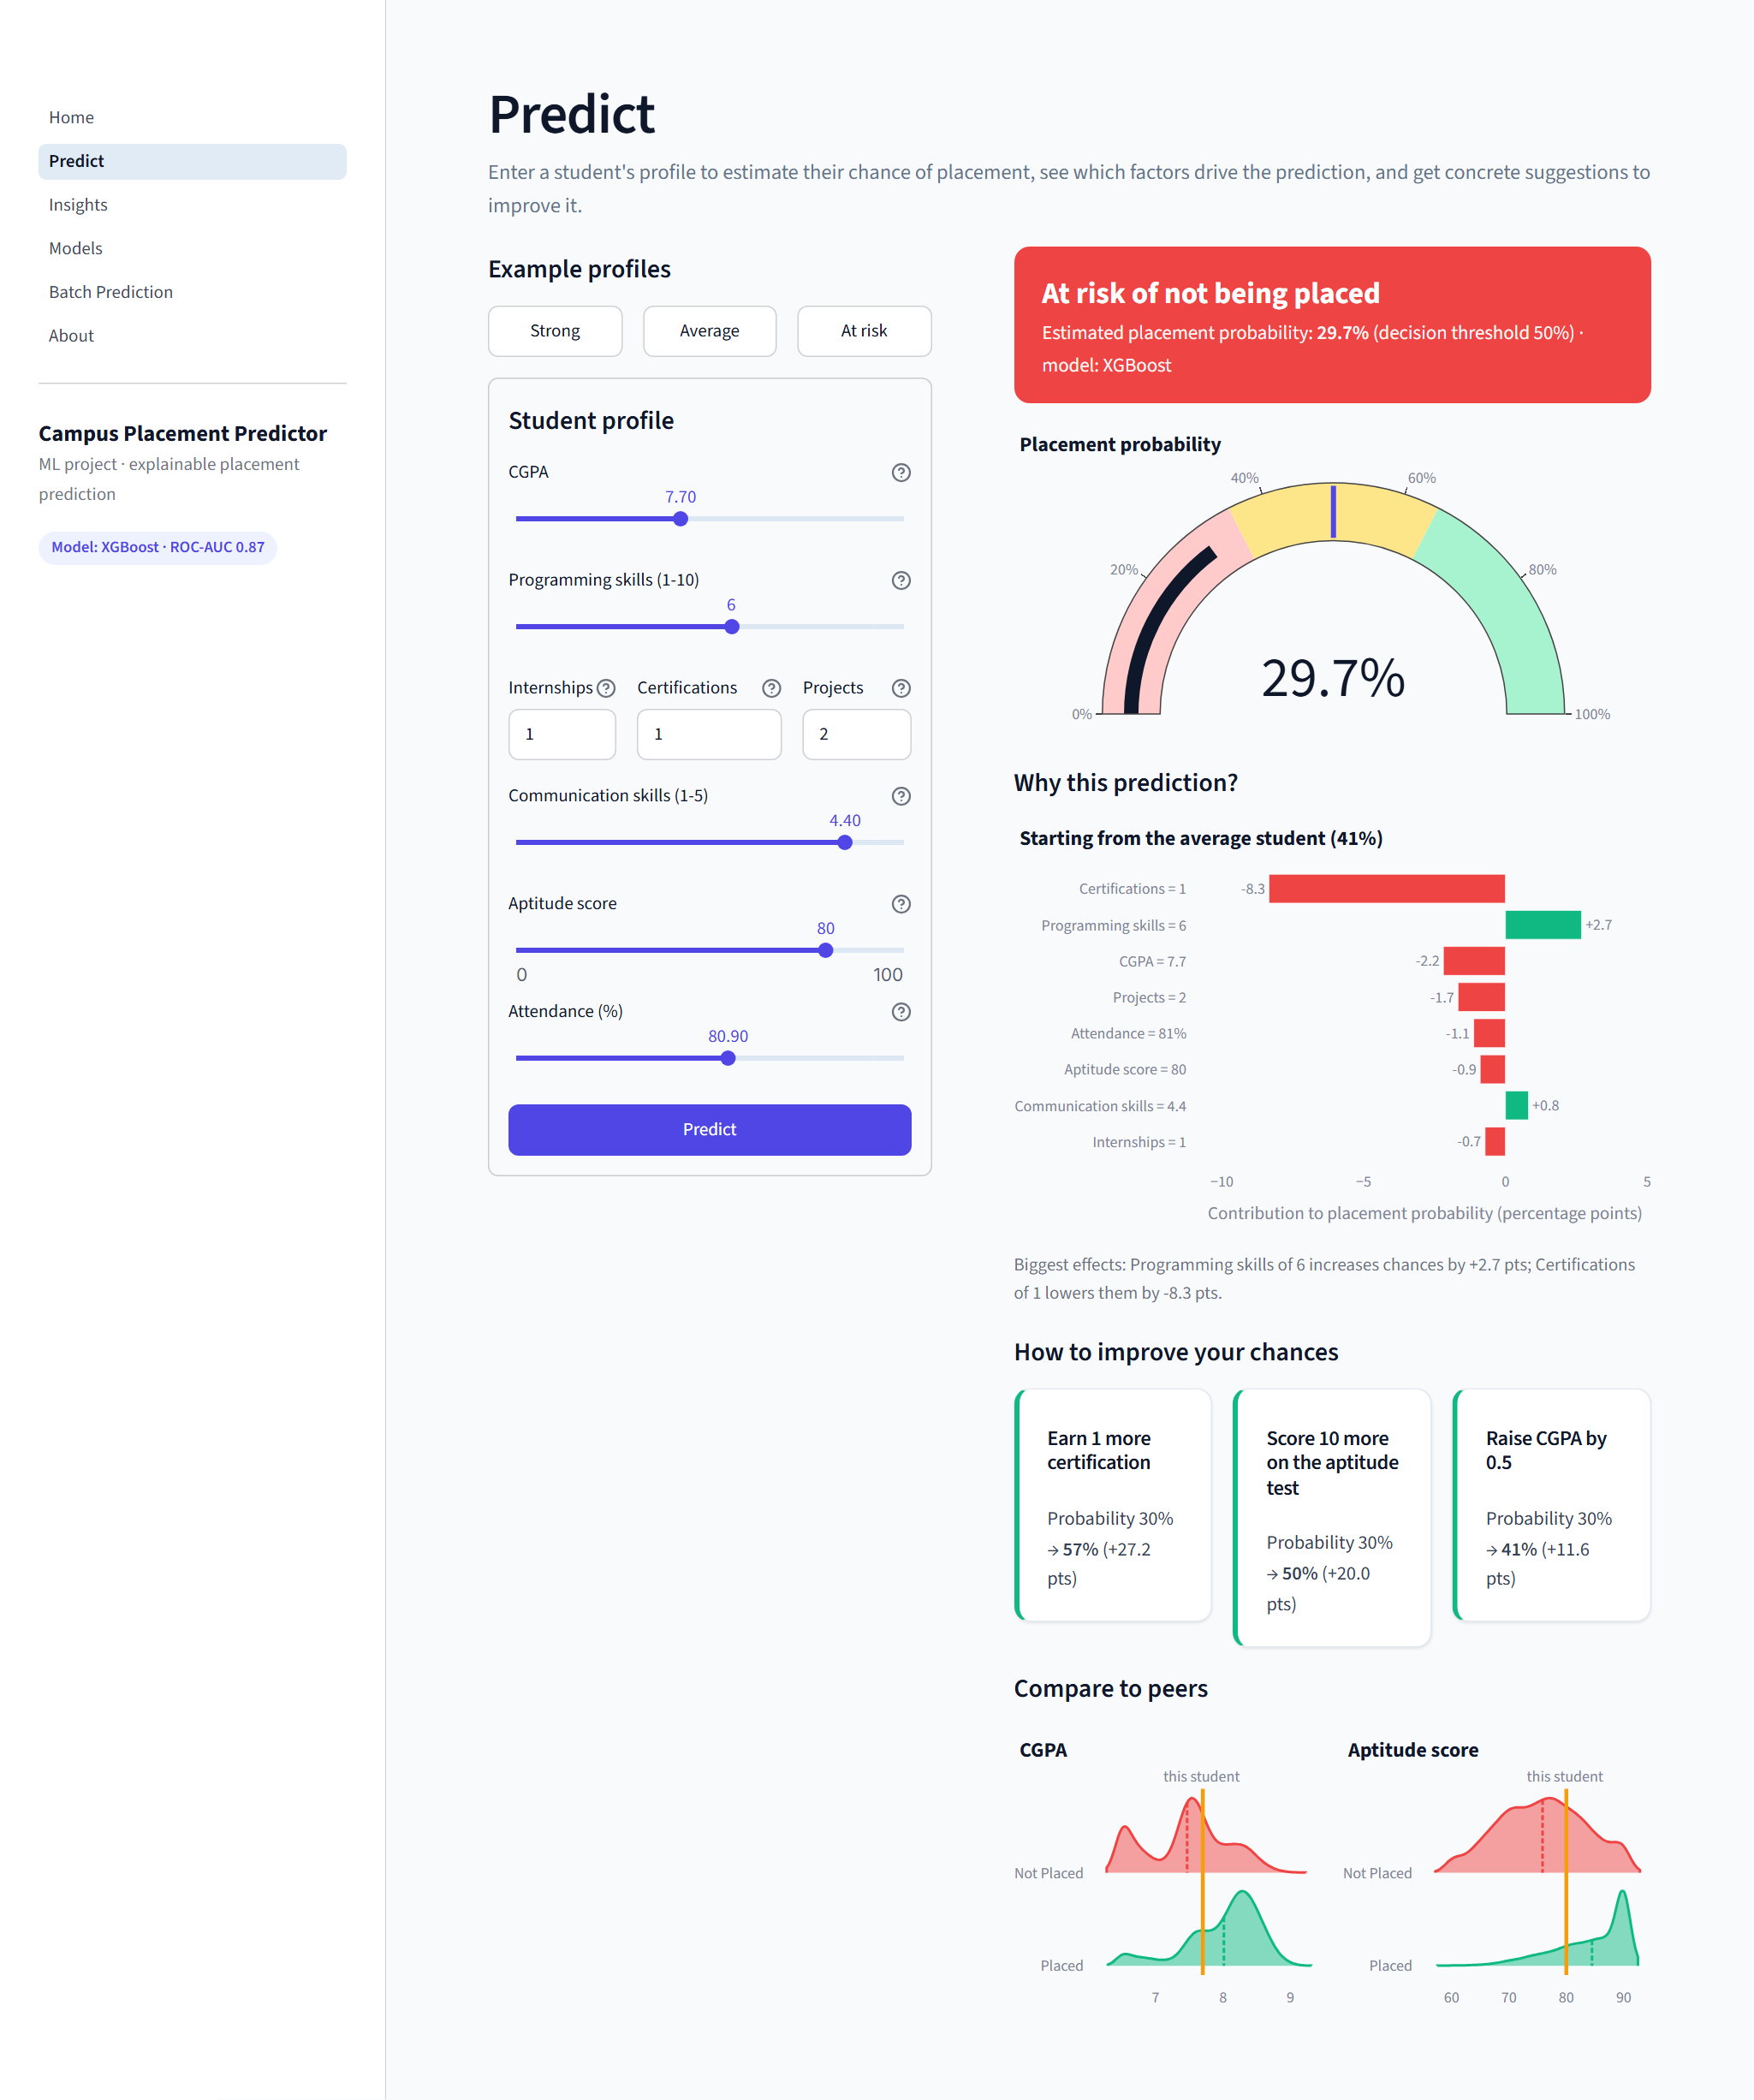
\includegraphics[width=\columnwidth]{predict.png}
\caption{Prediction page of the web application: verdict, probability gauge, SHAP explanation and what-if suggestions.}
\label{fig:app}
\end{figure}

% ===========================================================================
\section{Model Development}\label{sec:models}
Each model is a complete scikit-learn~\cite{pedregosa2011sklearn} pipeline (imputer $\rightarrow$ [scaler]
$\rightarrow$ classifier), tuned on the training set. The tuned hyper-parameters are listed in
Table~\ref{tab:hp}.
\begin{itemize}
  \item \textbf{Logistic Regression (LR)}: an interpretable baseline whose coefficients give direct influence
        estimates and odds ratios.
  \item \textbf{K-Nearest Neighbours (KNN)}~\cite{cover1967knn}: a simple non-parametric, instance-based comparison.
  \item \textbf{Support Vector Machine (SVM)}~\cite{cortes1995svm} with an RBF kernel: strong on medium-sized
        tabular data with non-linear class boundaries.
  \item \textbf{Random Forest (RF)}~\cite{breiman2001rf}: a robust bagged tree ensemble that captures
        non-linearity and provides impurity-based importance.
  \item \textbf{\XGBName{}}~\cite{chen2016xgboost}: regularised gradient-boosted trees, a state-of-the-art method
        for tabular data.
\end{itemize}

\begin{table}[t]
\centering
\caption{Tuned hyper-parameters}
\label{tab:hp}
\footnotesize
\begin{tabular}{p{0.24\columnwidth}p{0.68\columnwidth}}
\toprule
Model & Tuned hyper-parameters (best of RandomizedSearchCV) \\
\midrule
Logistic Regression & C=1.24, penalty=l2 \\
KNN & n\_neighbors=136, p=1, weights=distance \\
SVM (RBF) & C=0.534, gamma=0.00748 \\
Random Forest & max\_depth=10, max\_features=sqrt, min\_samples\_leaf=1, n\_estimators=353 \\
XGBoost & colsample\_bytree=0.743, learning\_rate=0.026, max\_depth=5, min\_child\_weight=13, n\_estimators=140, reg\_lambda=0.391, subsample=0.666 \\
\bottomrule
\end{tabular}

\end{table}

% ===========================================================================
\section{Results and Interpretation}\label{sec:results}
\subsection{Model comparison}
Table~\ref{tab:results} reports test-set metrics and cross-validated ROC-AUC. \BestModel{} has the highest mean
CV ROC-AUC (\BestCVAUC{}~$\pm$~\BestCVAUCsd{}) and is therefore selected. Selection uses cross-validation rather
than the test score, so the test set remains an unbiased estimate. On the test set \BestModel{} achieves
ROC-AUC \BestTestAUC{}, PR-AUC \BestTestPRAUC{}, accuracy \BestTestAcc{}, precision \BestTestPrec{}, recall
\BestTestRec{}, F1 \BestTestF{} and MCC \BestTestMCC{}. All five models lie within \CVAUCRange{} CV ROC-AUC of each
other (lowest: \WorstModel{}, \WorstCVAUC{}), and their ROC curves almost overlap (Fig.~\ref{fig:roc}). This
indicates that the signal in the data is largely monotonic and is captured equally well by linear and
non-linear models. The confusion matrices (Fig.~\ref{fig:cm}) show that the dominant error type is missing placed
students (false negatives) at the default threshold.

\begin{table*}[t]
\centering
\caption{Test-set performance and 5-fold CV ROC-AUC (best value per column in bold; $^\star$ = selected model)}
\label{tab:results}
\scriptsize
\setlength{\tabcolsep}{3pt}
\begin{tabular}{lrrrrrrrrr}
\toprule
Model & Acc & Prec & Rec & F1 & ROC & PR & MCC & CV ROC-AUC & Time (s) \\
\midrule
XGBoost$^\star$ & 0.797 & 0.777 & 0.726 & 0.750 & \textbf{0.869} & 0.834 & 0.581 & \textbf{0.865$\pm$0.005} & 10 \\
Random Forest & 0.791 & 0.772 & 0.712 & 0.741 & 0.865 & 0.826 & 0.567 & 0.864$\pm$0.005 & 29 \\
SVM (RBF) & \textbf{0.802} & \textbf{0.789} & 0.722 & 0.754 & 0.868 & \textbf{0.838} & \textbf{0.591} & 0.862$\pm$0.005 & 35 \\
Logistic Regression & 0.799 & 0.770 & \textbf{0.745} & \textbf{0.757} & 0.866 & 0.838 & 0.587 & 0.861$\pm$0.005 & 8 \\
KNN & 0.798 & 0.776 & 0.731 & 0.753 & 0.864 & 0.821 & 0.584 & 0.860$\pm$0.005 & 5 \\
\bottomrule
\end{tabular}

\end{table*}

\begin{figure}[t]
\centering
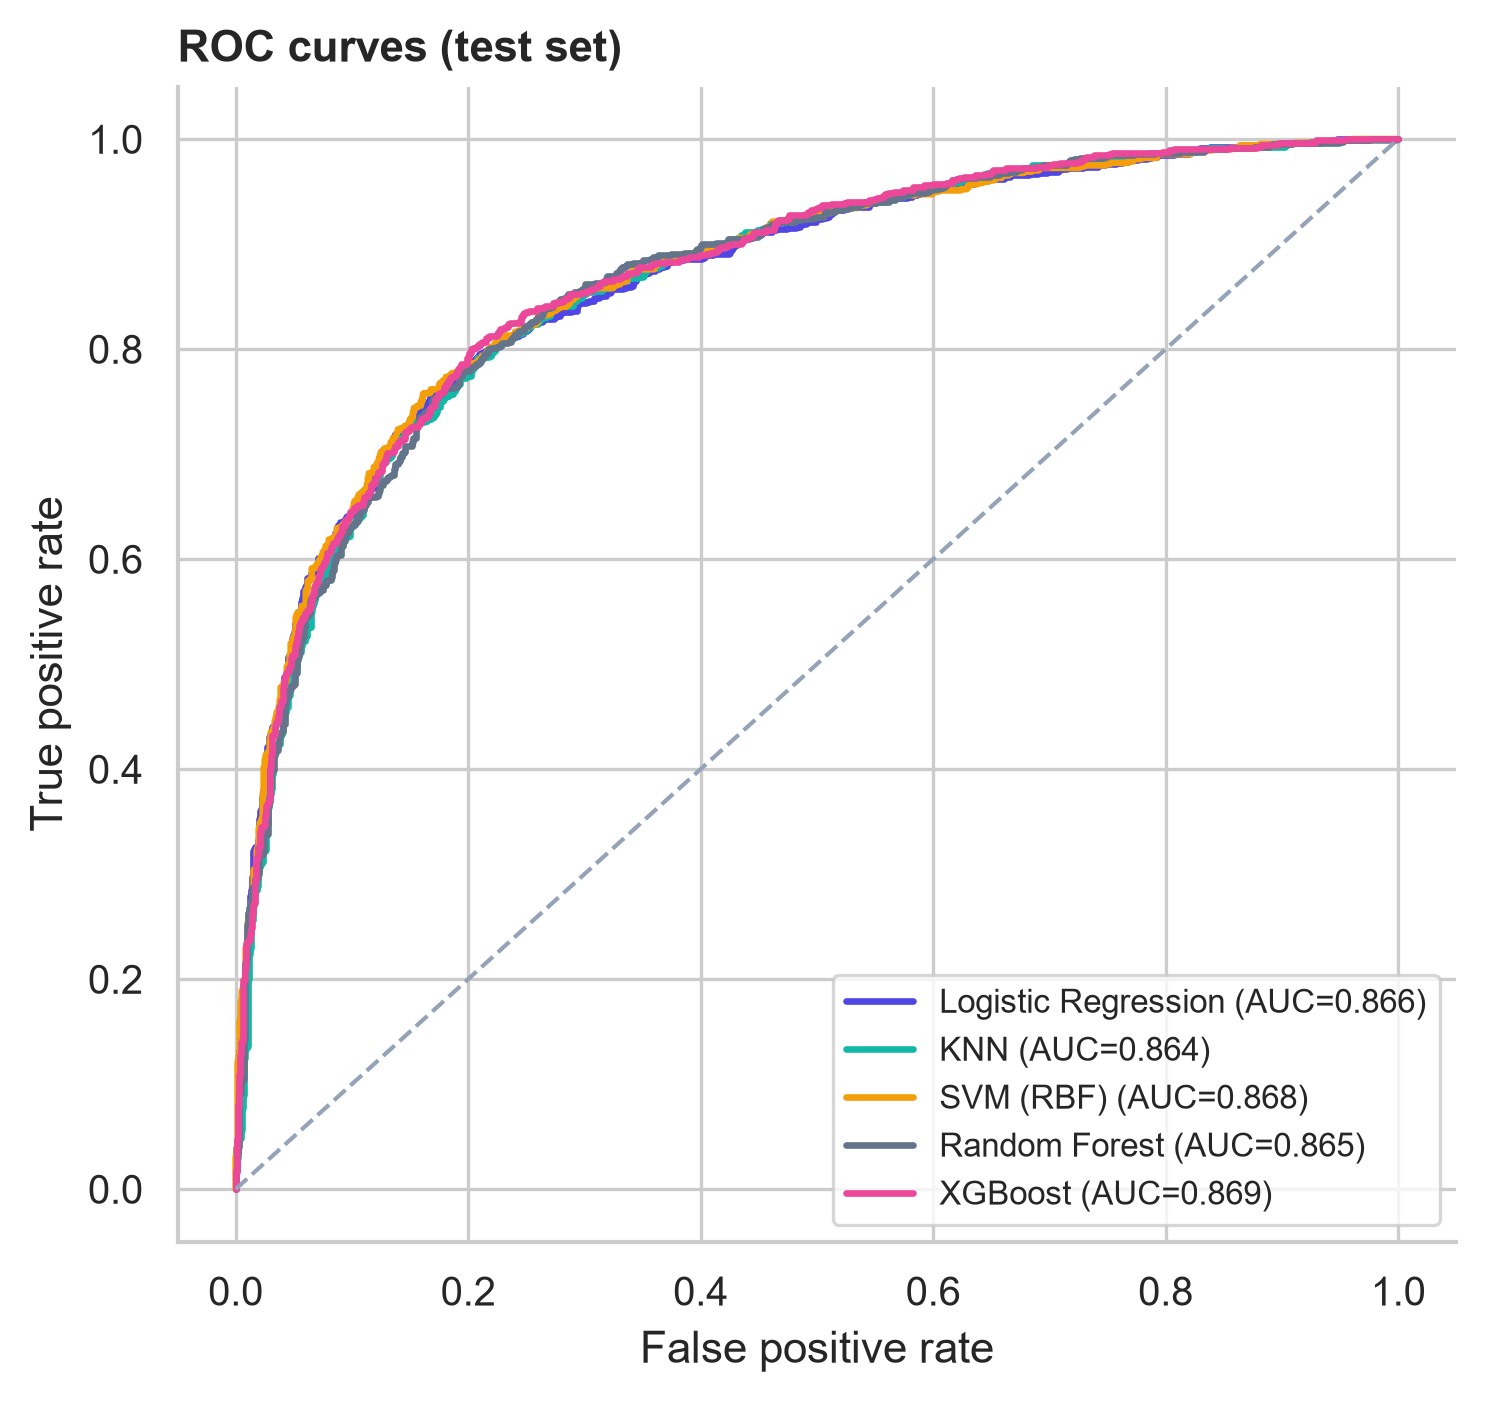
\includegraphics[width=0.49\columnwidth]{roc_curves.png}\hfill
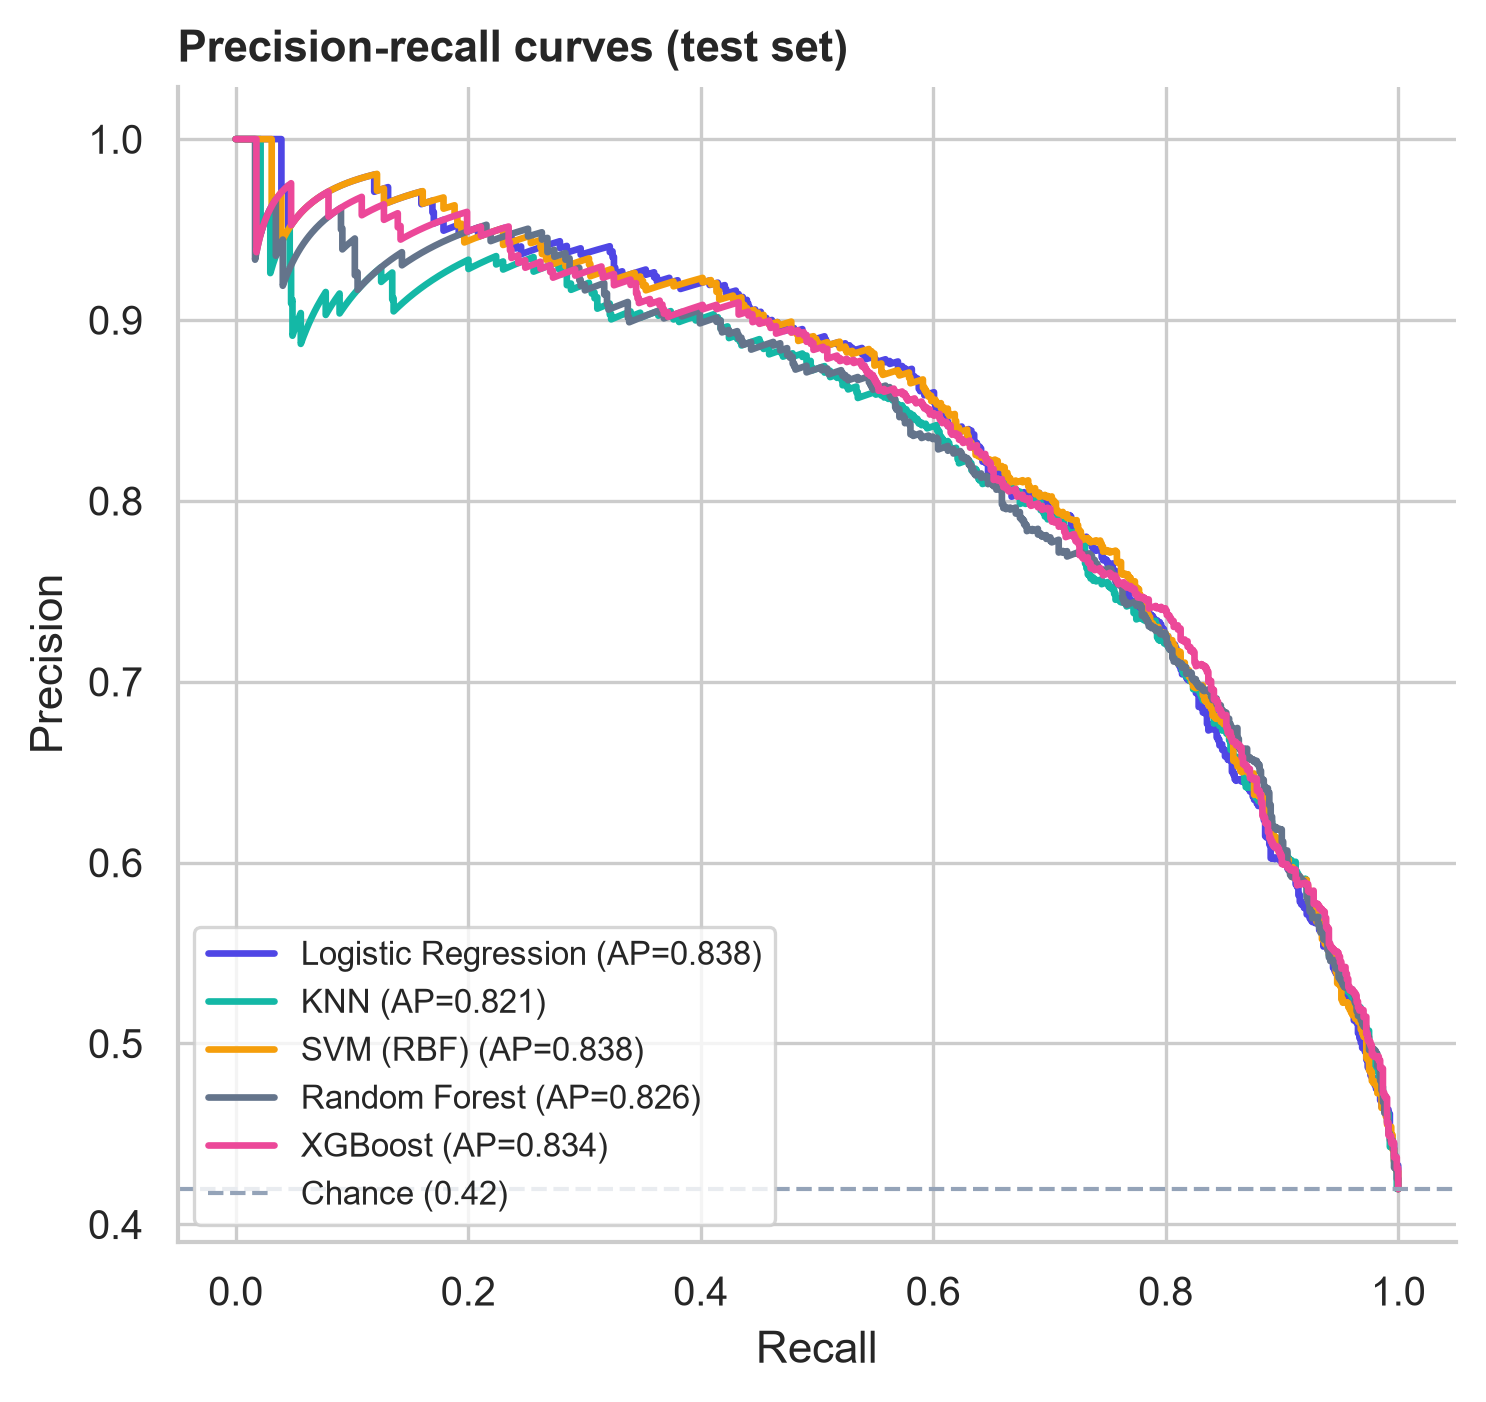
\includegraphics[width=0.49\columnwidth]{pr_curves.png}
\caption{ROC (left) and precision--recall (right) curves on the test set.}
\label{fig:roc}
\end{figure}

\begin{figure*}[t]
\centering
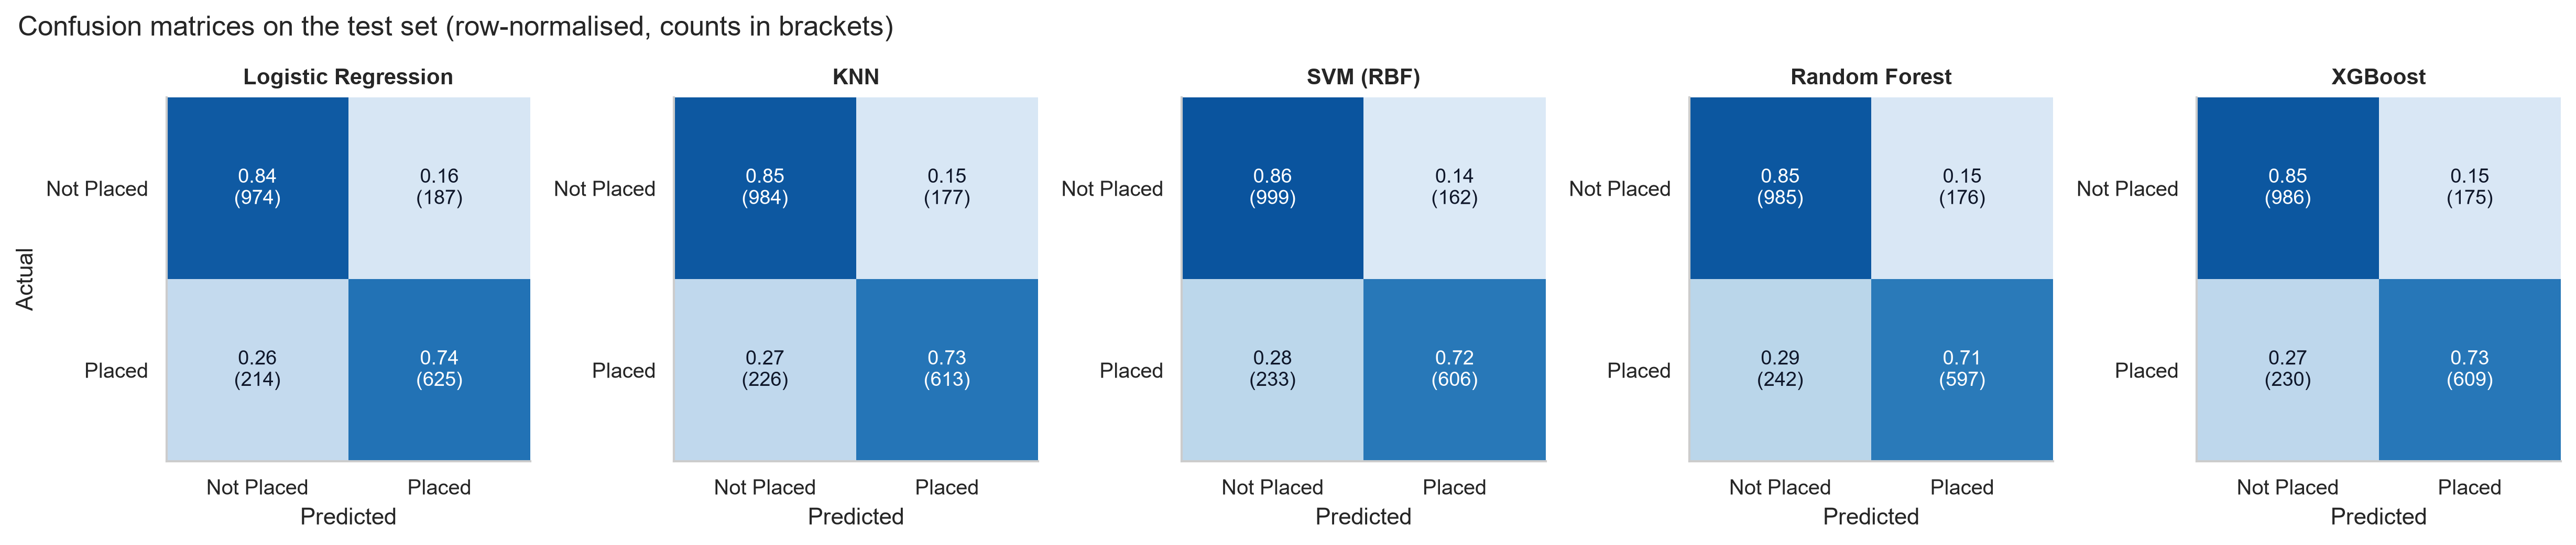
\includegraphics[width=0.95\textwidth]{confusion_matrices.png}
\caption{Row-normalised confusion matrices on the test set (counts in brackets).}
\label{fig:cm}
\end{figure*}

\begin{figure}[t]
\centering
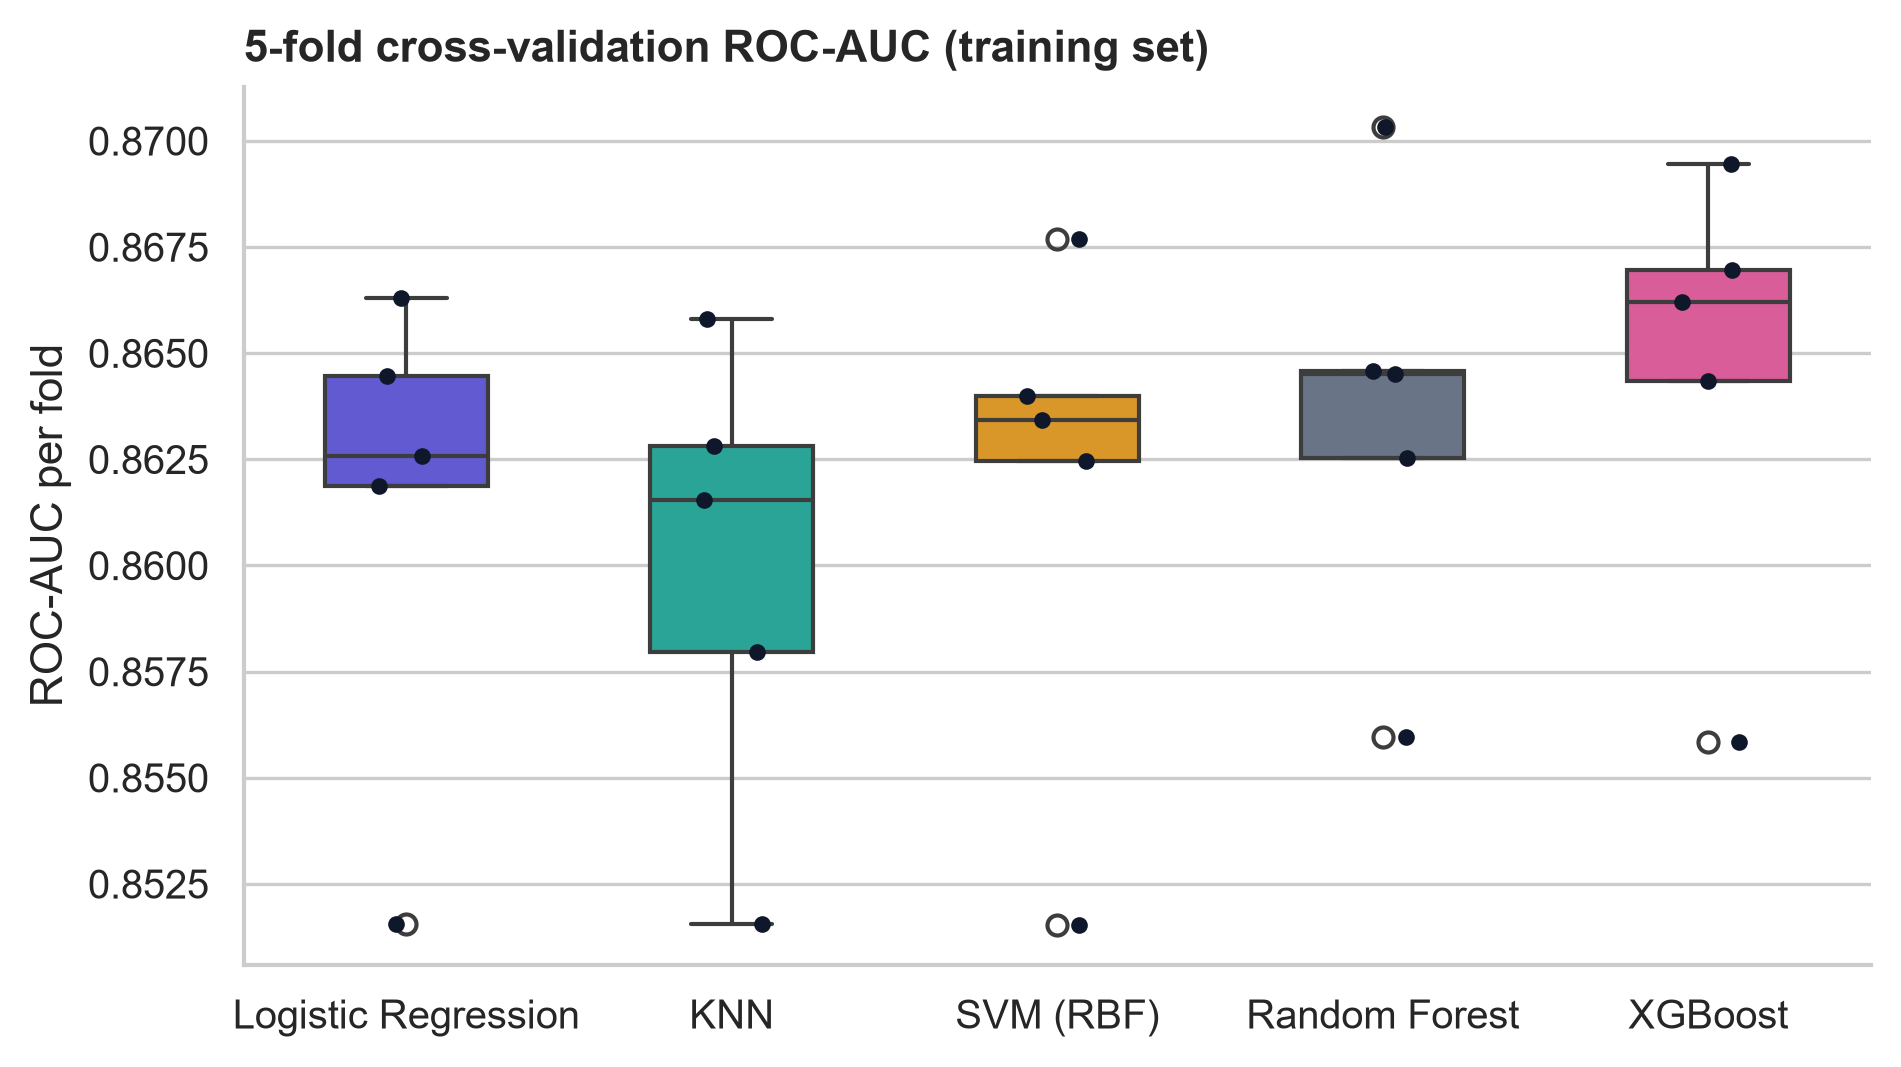
\includegraphics[width=\columnwidth]{cv_boxplot.png}
\caption{Distribution of ROC-AUC over the five cross-validation folds.}
\label{fig:cv}
\end{figure}

\subsection{Statistical significance}
\BestModel{} and the runner-up \SecondModel{} were compared on the same five folds (Fig.~\ref{fig:cv}). The mean
difference in ROC-AUC is \StatDiff{}; a paired $t$-test gives $p=\StatP{}$ and the Nadeau--Bengio corrected
test~\cite{nadeau2003inference}, which accounts for overlapping training sets, gives $p=\StatPcorr{}$.
McNemar's test~\cite{mcnemar1947} on the test predictions gives $p=\McNemarP{}$. The difference therefore
\StatSig{} significant at the 5\% level: the two ensembles perform practically the same, and the choice
between them can be based on secondary criteria such as training time and model size.

\subsection{Calibration and learning behaviour}
The calibration curve of \BestModel{} (Fig.~\ref{fig:calib}, left) follows the diagonal closely, so predicted
probabilities can be read as approximate placement chances, which matters for the gauge and the what-if panel
of the application. The learning curve (Fig.~\ref{fig:calib}, right) ends with a gap of \LCGap{} between
training and validation ROC-AUC, indicating mild overfitting. The validation score is still rising slowly at the
full training size, so additional data would bring small further gains.

\begin{figure}[t]
\centering
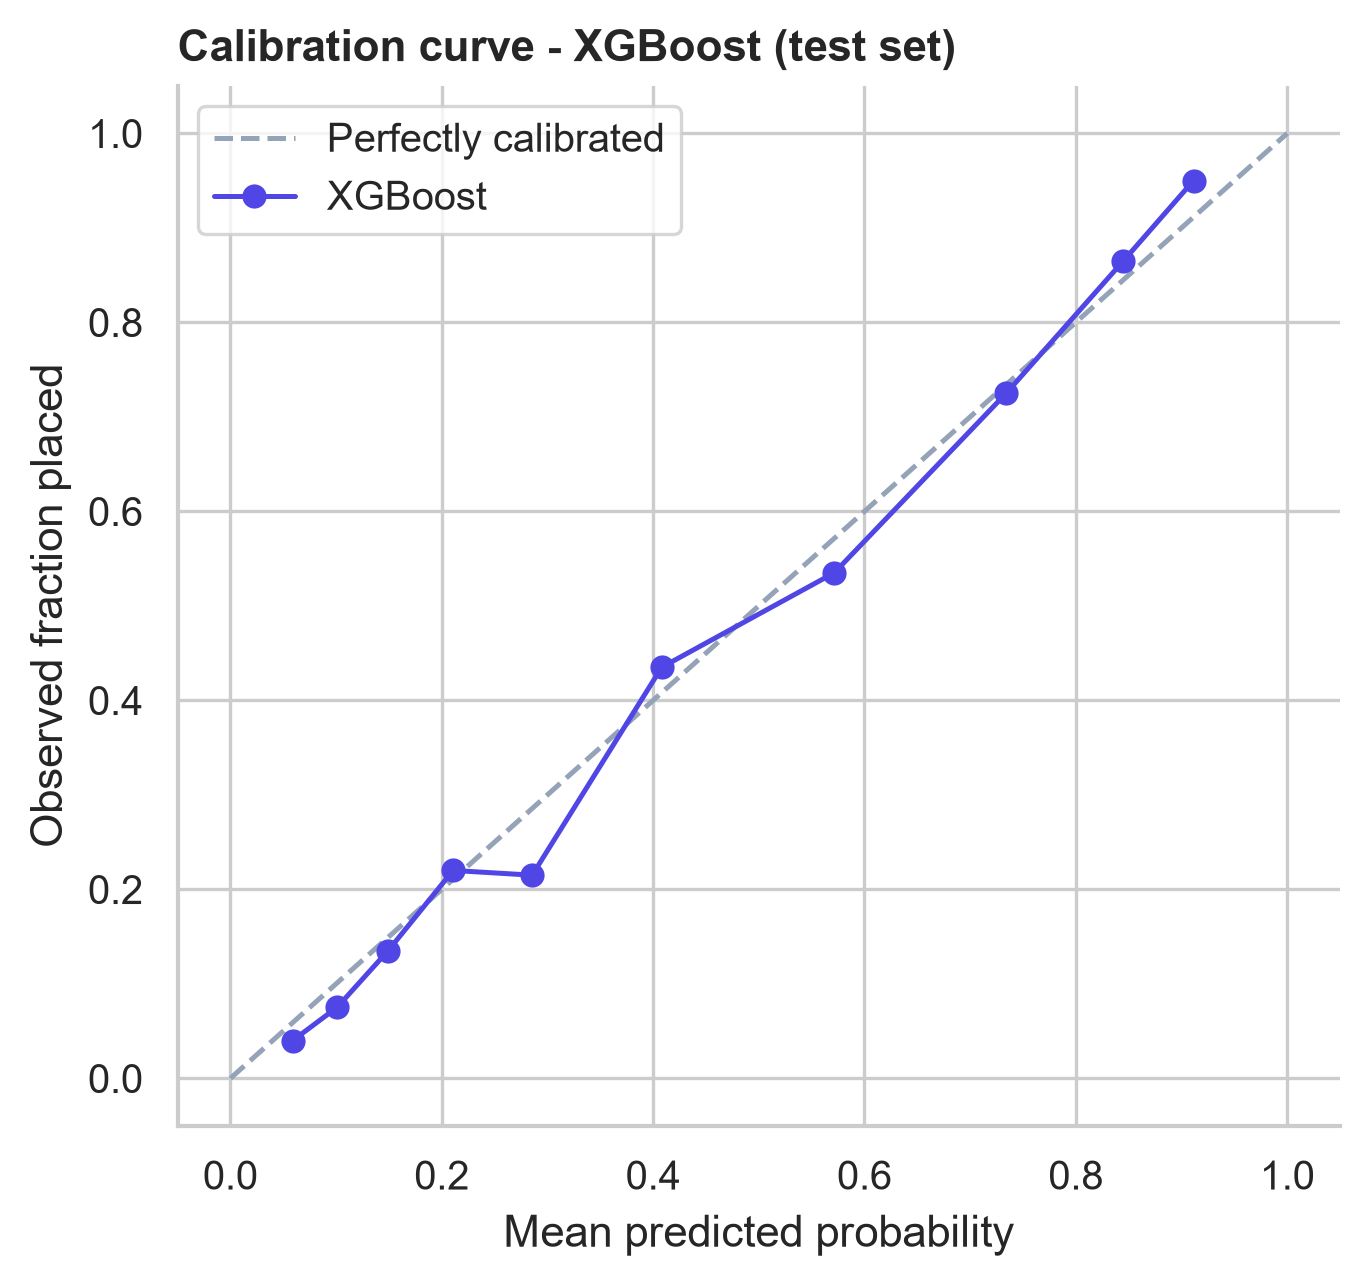
\includegraphics[width=0.49\columnwidth]{calibration_curve.png}\hfill
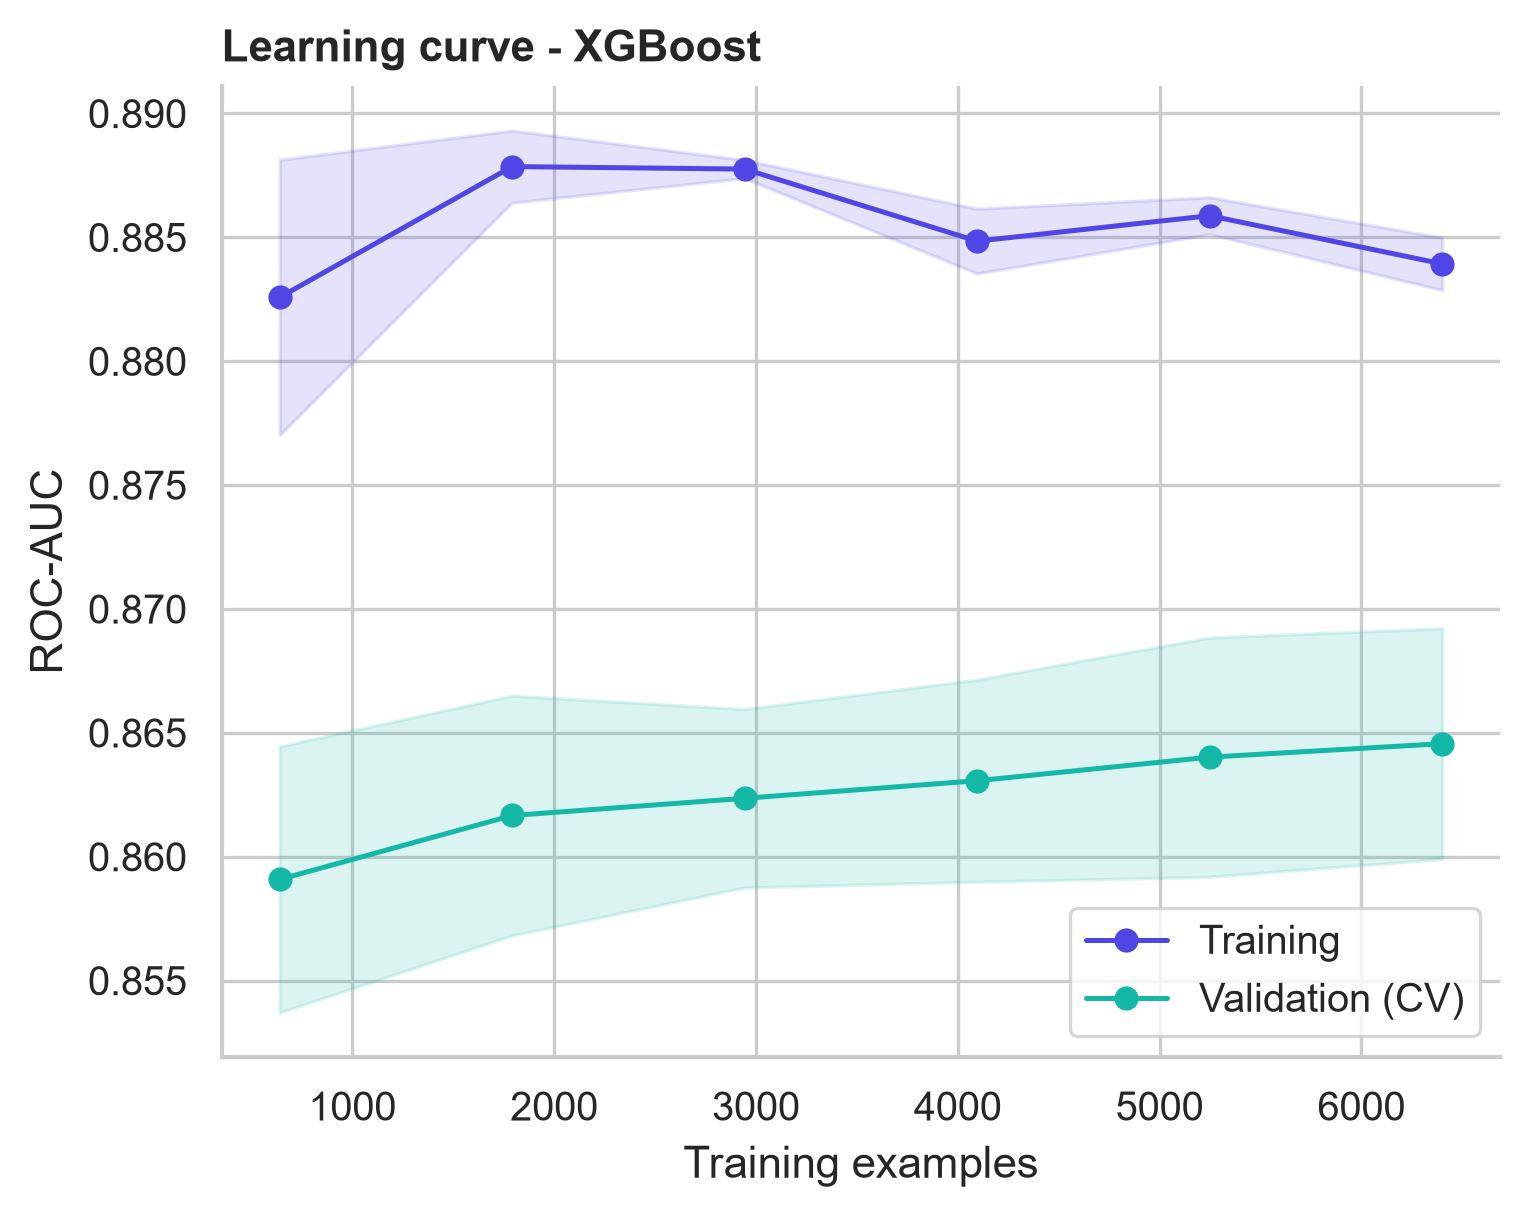
\includegraphics[width=0.49\columnwidth]{learning_curve.png}
\caption{Calibration curve (left) and learning curve (right) of the selected model.}
\label{fig:calib}
\end{figure}

\subsection{Influential features}
Five methods were used: absolute logistic-regression coefficients on standardised inputs, random-forest
impurity importance, \XGBName{} gain, permutation importance of the selected model on the test set (20 repeats),
and mean absolute SHAP values~\cite{lundberg2017shap} of the selected model in probability units. Each
importance vector was normalised and the features were ranked by their mean rank (Table~\ref{tab:fi},
Fig.~\ref{fig:fi}).

\TopOne{} is the most influential attribute, followed by \TopTwo{} and \TopThree{}; \LeastFeature{} is the least
influential. In the logistic model a one-standard-deviation increase in \OddsTopFeature{} multiplies the odds of
placement by \OddsTop{} (Fig.~\ref{fig:lr}). The SHAP summary (Fig.~\ref{fig:shap}) shows that high values of
the top attributes consistently push the prediction towards \emph{placed}. Partial dependence
plots~\cite{friedman2001pdp} (Fig.~\ref{fig:pdp}) show the shape of these effects. The findings generated
automatically from the numbers are:
\begin{itemize}
\item AptitudeScore is the most influential feature overall (consensus rank 1; ranked first by 4 of 5 methods).
\item The three most influential features are AptitudeScore, ProgrammingSkills and Certifications.
\item Average placement probability rises from 21\% at AptitudeScore = 63 to 55\% at AptitudeScore = 90; the steepest change is between 89 and 90.
\item Average placement probability rises from 32\% at ProgrammingSkills = 1 to 51\% at ProgrammingSkills = 10; the steepest change is between 4 and 5.
\item Average placement probability rises from 38\% at Certifications = 0 to 46\% at Certifications = 3; the steepest change is between 1 and 2.
\item In the logistic regression model, a one-standard-deviation increase in AptitudeScore multiplies the odds of placement by 2.06.
\item Internships has a negative coefficient in the logistic model: holding the other features fixed, higher values slightly reduce the odds of placement (odds ratio 0.94).
\item The five importance methods agree moderately on the ranking: mean pairwise Spearman rank correlation = 0.60.
\item Internships is the least influential feature (consensus rank 8).
\item The simulated columns rank ProgrammingSkills \#2 and Attendance \#7 (their influence reflects the simulation formula, not real evidence); removing both has only a small effect on CV ROC-AUC (-0.0081).
\item Adding the extra Kaggle columns (extracurriculars, placement training, SSC/HSC marks) changes CV ROC-AUC by +0.0185; they are left out of the main model because the problem statement defines the 8 core features.
\item Engineered features changed CV ROC-AUC by -0.0008 (not used; rule: gain >= 0.005).
\end{itemize}


The methods agree moderately overall (mean pairwise Spearman $\rho=\MeanRho{}$, Table~\ref{tab:agree}).
Permutation importance and SHAP, which both explain the selected model, agree closely with each other and with
the logistic coefficients, whereas impurity-based importances favour attributes with many distinct split
points. This illustrates why a single importance method should not be relied upon.

Two cautions apply. First, the simulated \texttt{ProgrammingSkills} ranks \RankProg{} and the simulated
\texttt{Attendance} ranks \RankAtt{}; their influence is a consequence of the simulation formulas. Second,
\LeastFeature{} has little influence once the other attributes are known, even though placement rate rises
with it in isolation (Fig.~\ref{fig:bins}); its information is largely shared with the simulated programming score, which was
generated partly from internships ($r=\CorrInternProg{}$ in Fig.~\ref{fig:eda}b), so this result is partly an artefact of
the simulation.

\begin{table}[t]
\centering
\caption{Consensus feature ranking (rank per method; $^\dagger$ = simulated)}
\label{tab:fi}
\footnotesize
\setlength{\tabcolsep}{3pt}
\begin{tabular}{rlrrrrrrr}
\toprule
\# & Feature & LR & RF & XGB & Perm & SHAP & Mean & Score \\
\midrule
1 & AptitudeScore & 1 & 1 & 3 & 1 & 1 & 1.4 & 0.89 \\
2 & ProgrammingSkills$^\dagger$ & 2 & 5 & 4 & 2 & 2 & 3.0 & 0.45 \\
3 & Certifications & 5 & 3 & 2 & 4 & 3 & 3.4 & 0.47 \\
4 & CommunicationSkills & 3 & 7 & 5 & 3 & 4 & 4.4 & 0.38 \\
5 & Projects & 7 & 4 & 1 & 5 & 6 & 4.6 & 0.50 \\
6 & CGPA & 6 & 2 & 6 & 6 & 5 & 5.0 & 0.32 \\
7 & Attendance$^\dagger$ & 4 & 6 & 7 & 7 & 7 & 6.2 & 0.29 \\
8 & Internships & 8 & 8 & 8 & 8 & 8 & 8.0 & 0.07 \\
\bottomrule
\end{tabular}

\end{table}

\begin{table}[t]
\centering
\caption{Agreement between importance methods (Spearman $\rho$)}
\label{tab:agree}
\footnotesize
\setlength{\tabcolsep}{3pt}
\begin{tabular}{lrrrrr}
\toprule
 & LR & RF & XGB & Perm & SHAP \\
\midrule
LR & 1.00 & 0.31 & 0.21 & 0.83 & 0.81 \\
RF & 0.31 & 1.00 & 0.57 & 0.48 & 0.62 \\
XGB & 0.21 & 0.57 & 1.00 & 0.62 & 0.57 \\
Perm & 0.83 & 0.48 & 0.62 & 1.00 & 0.95 \\
SHAP & 0.81 & 0.62 & 0.57 & 0.95 & 1.00 \\
\bottomrule
\end{tabular}

\end{table}

\begin{figure}[t]
\centering
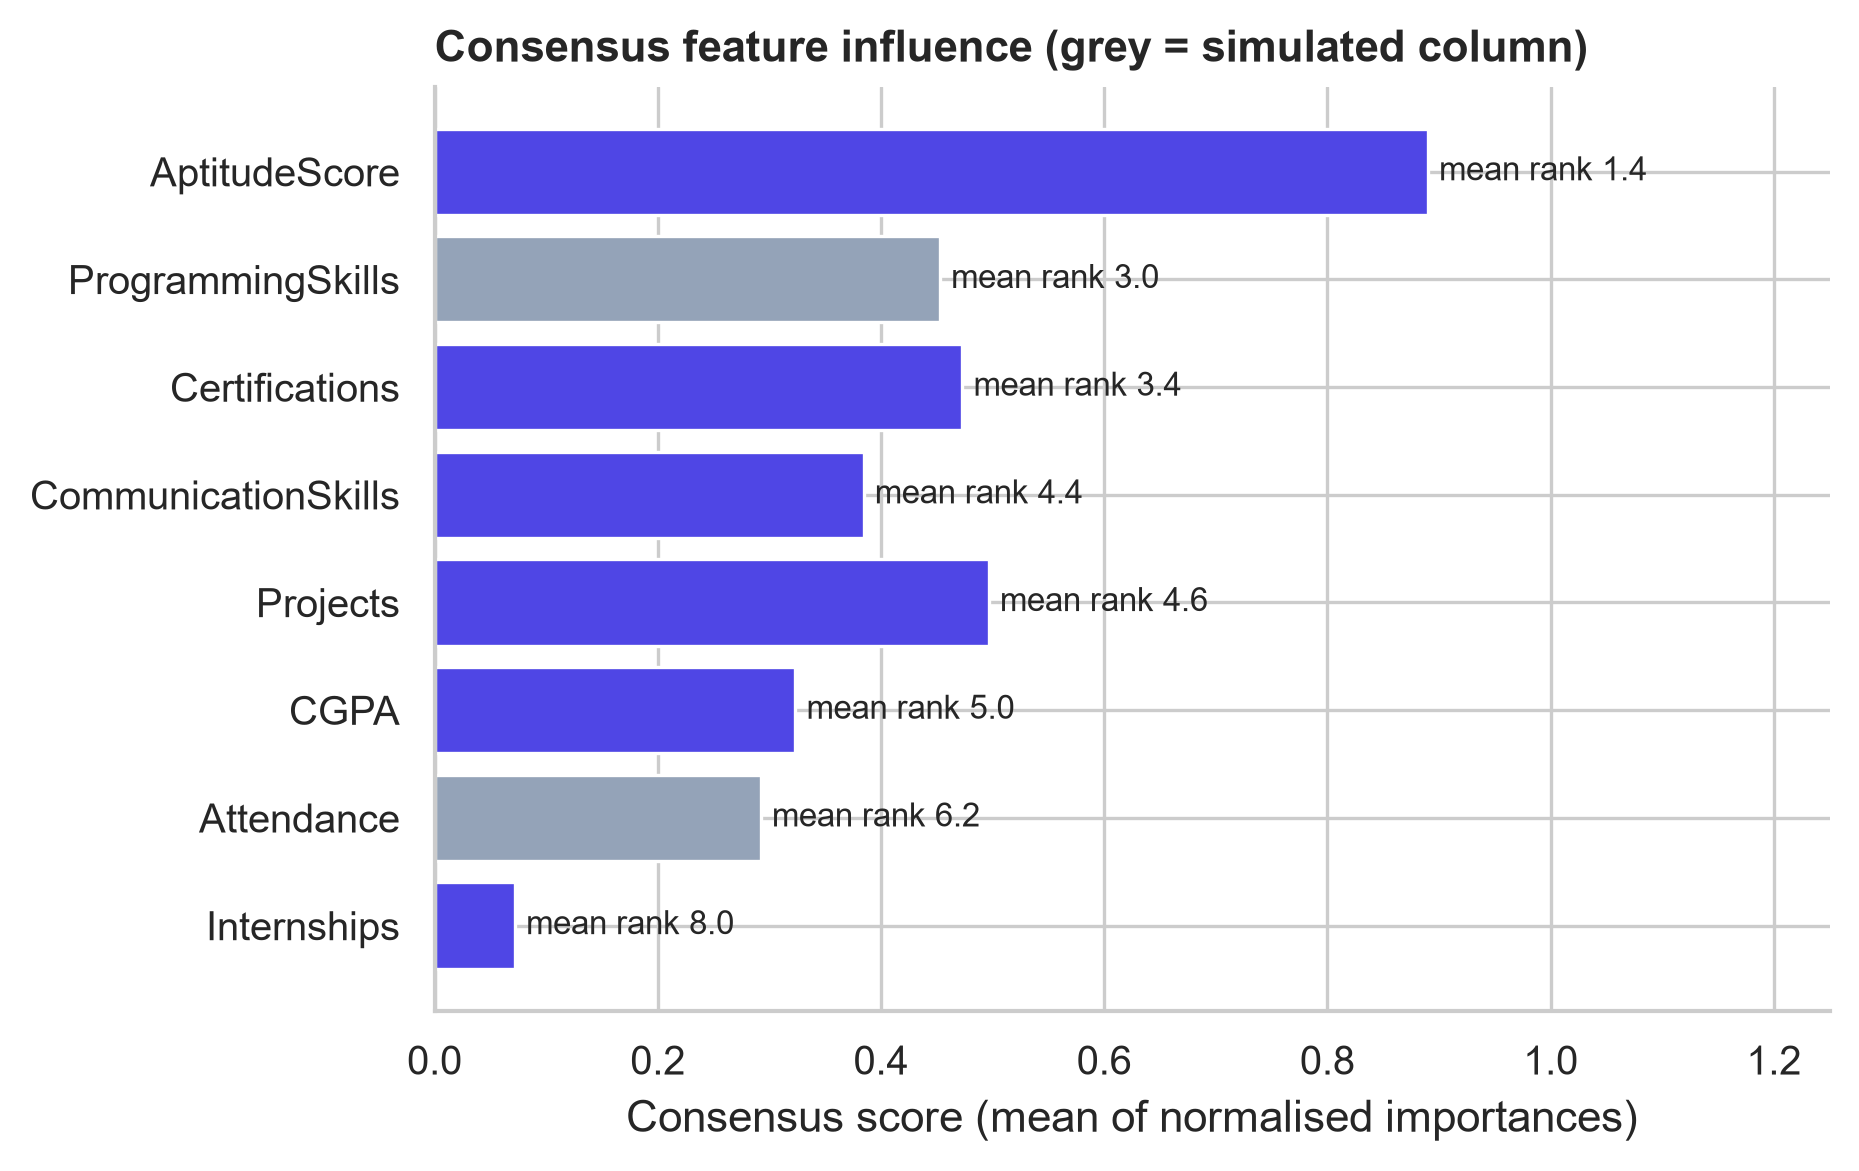
\includegraphics[width=\columnwidth]{feature_importance_consensus.png}
\caption{Consensus feature influence over five methods (grey = simulated attribute).}
\label{fig:fi}
\end{figure}

\begin{figure}[t]
\centering
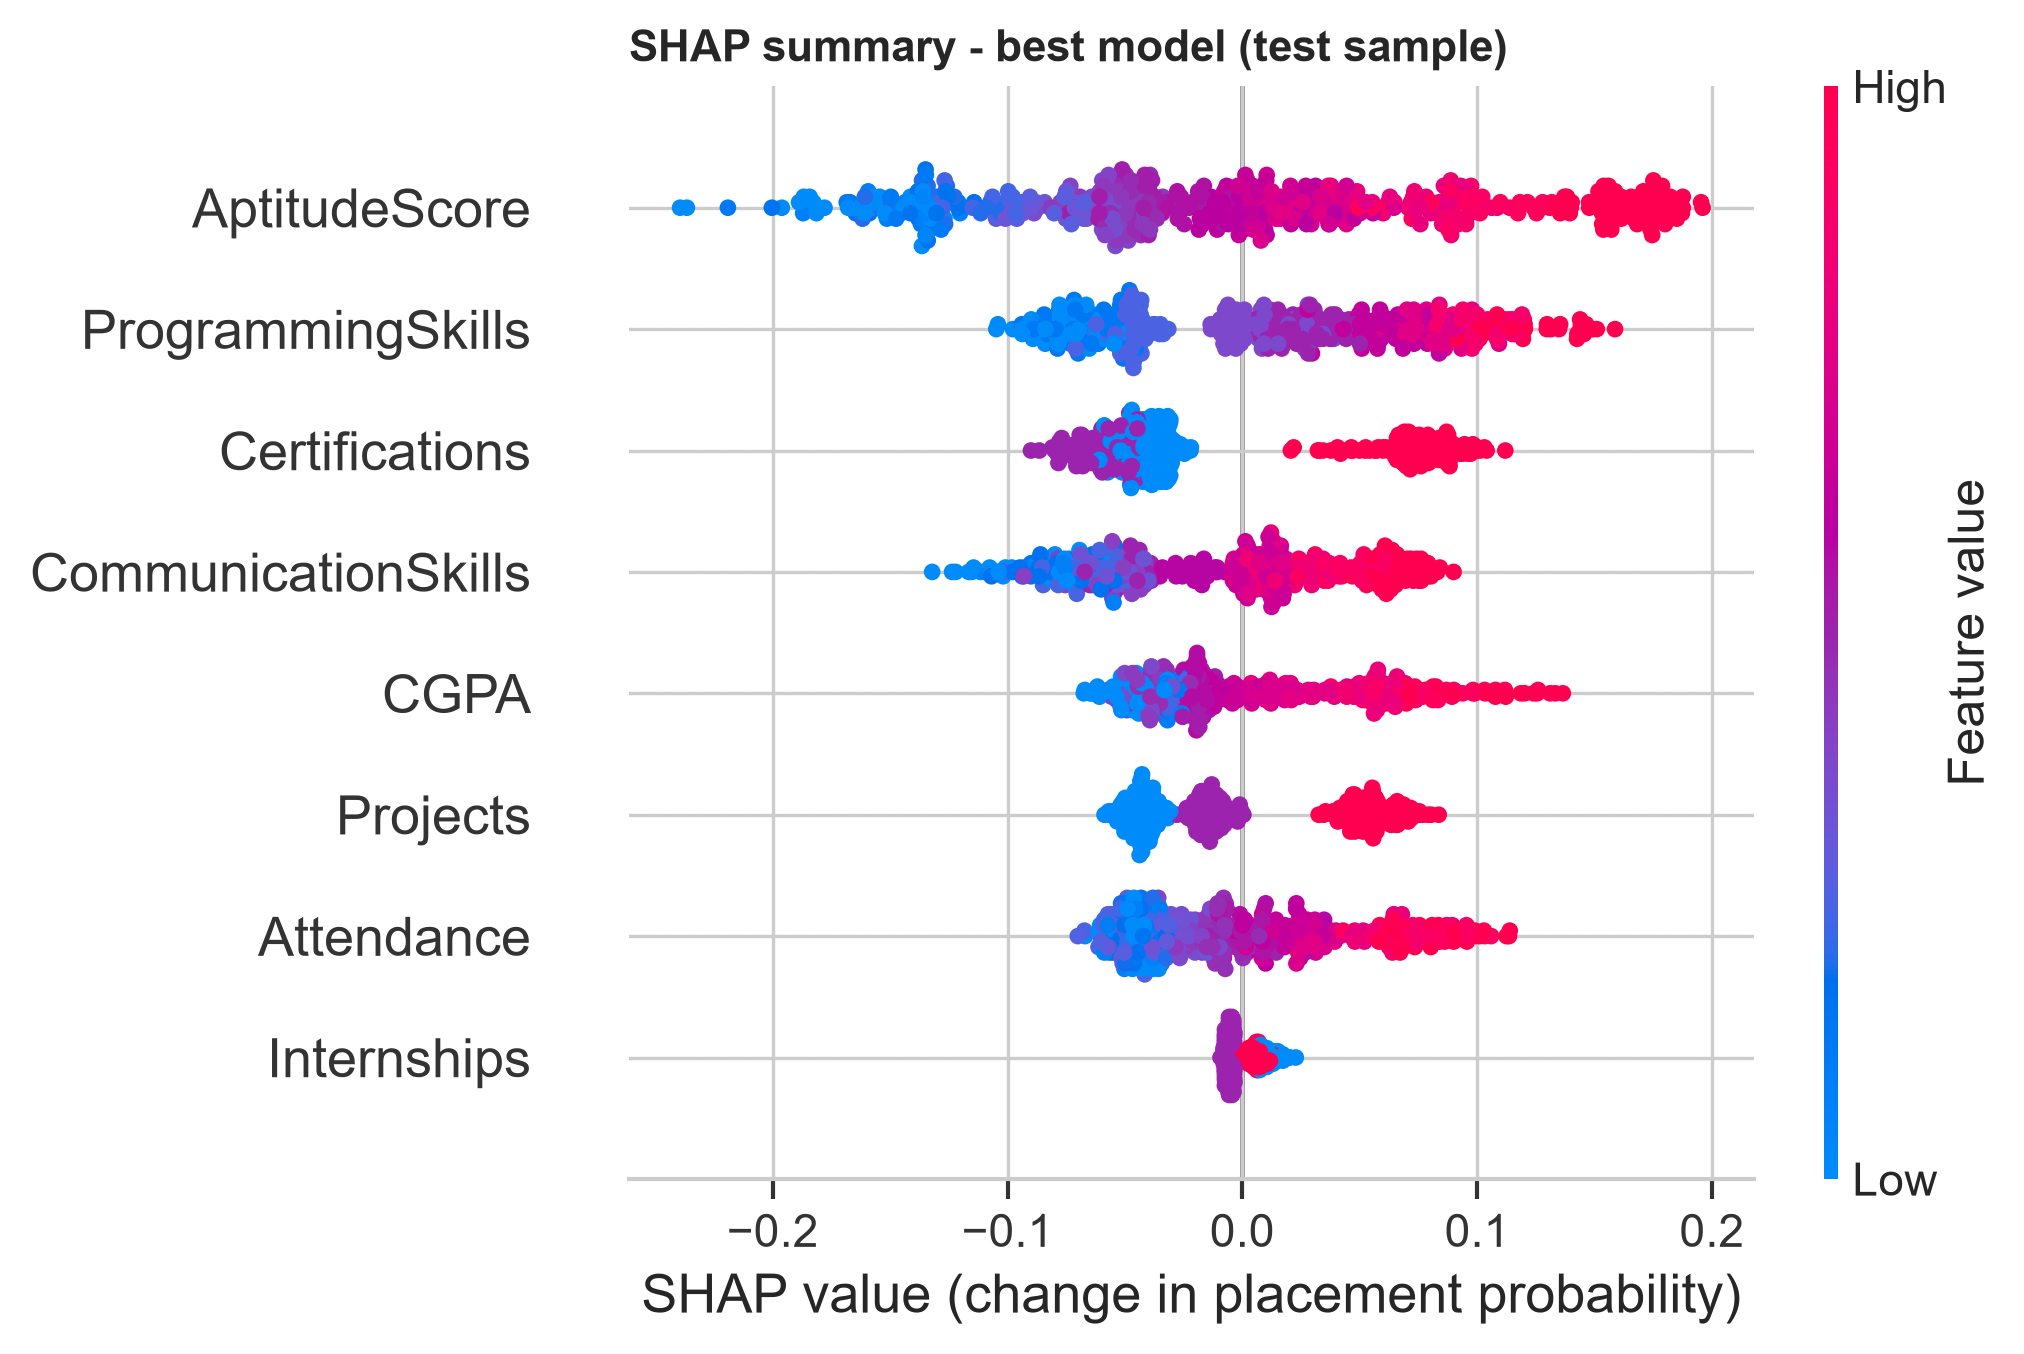
\includegraphics[width=\columnwidth]{shap_summary_beeswarm.png}
\caption{SHAP summary of the selected model on a test sample.}
\label{fig:shap}
\end{figure}

\begin{figure}[t]
\centering
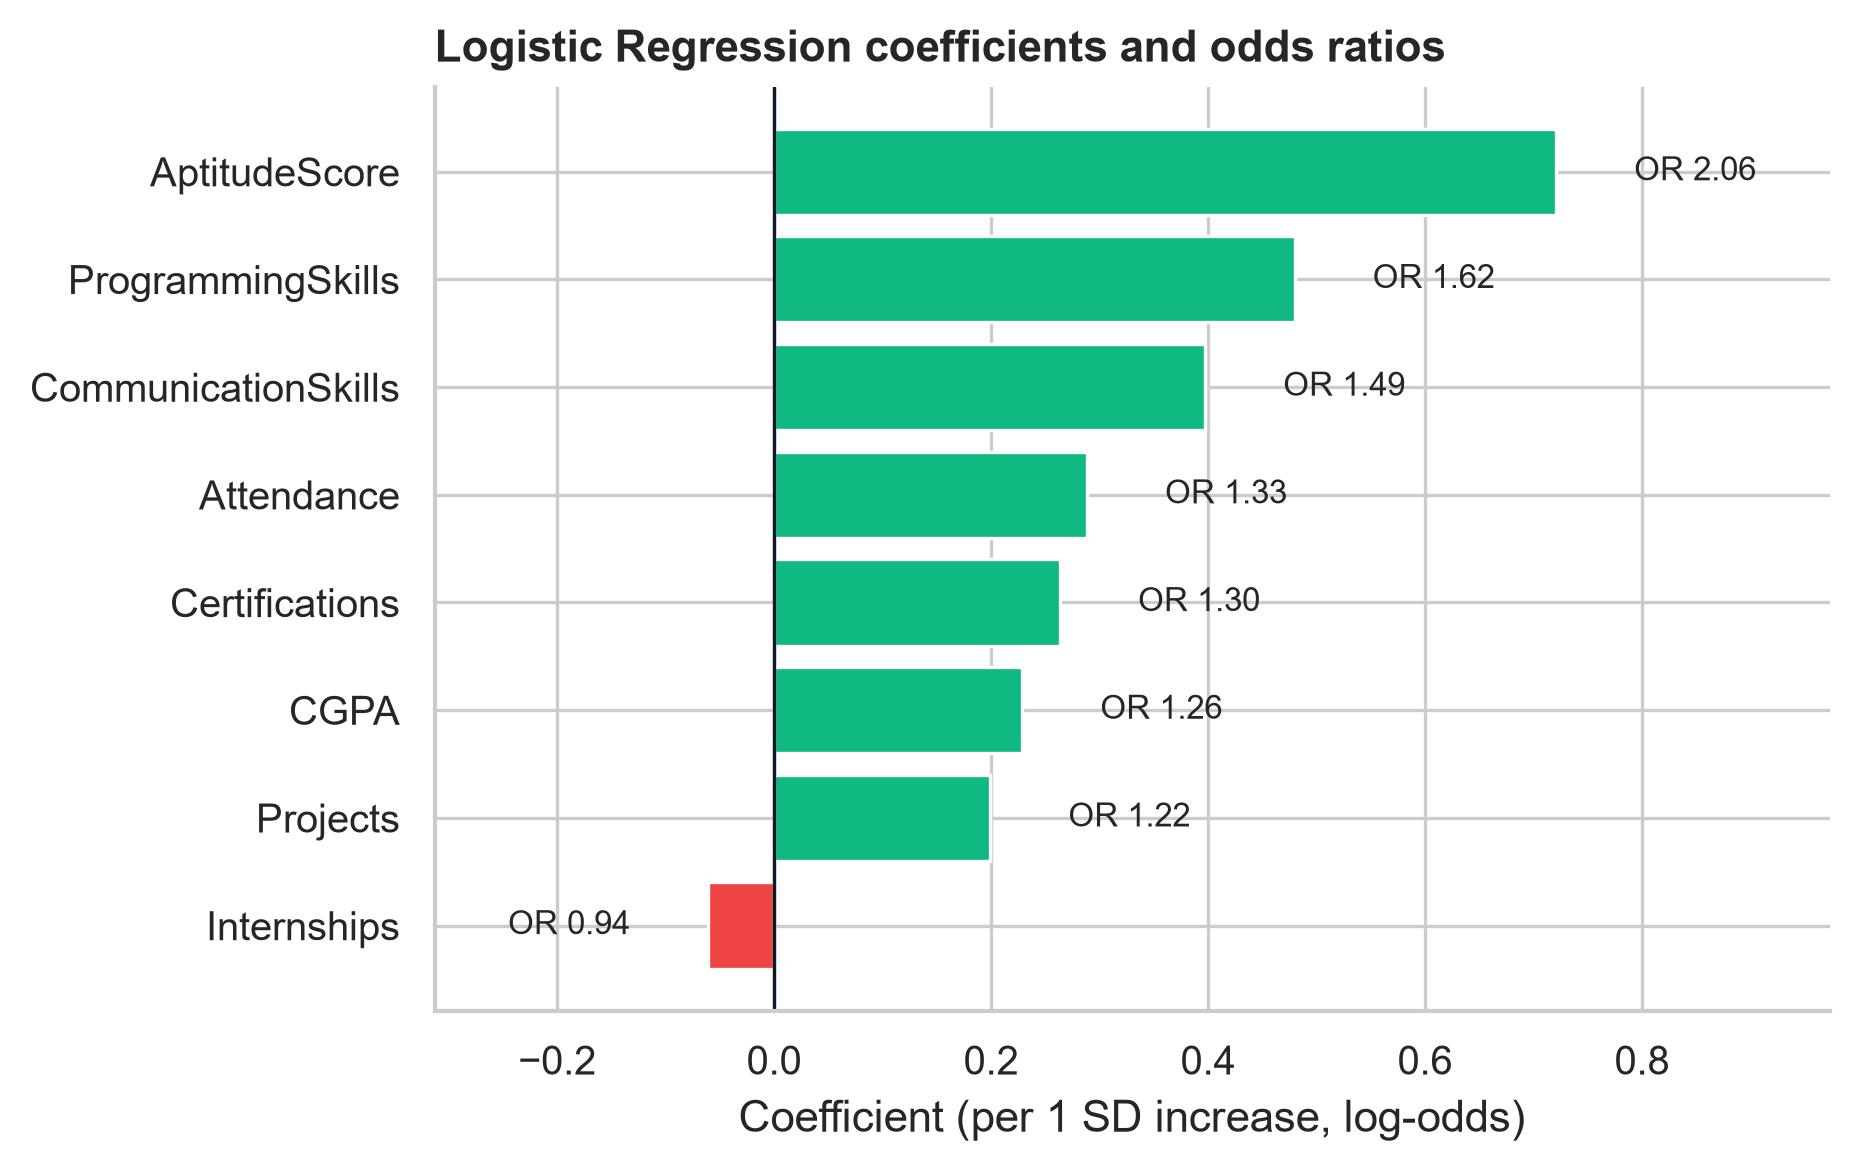
\includegraphics[width=0.49\columnwidth]{lr_coefficients.png}\hfill
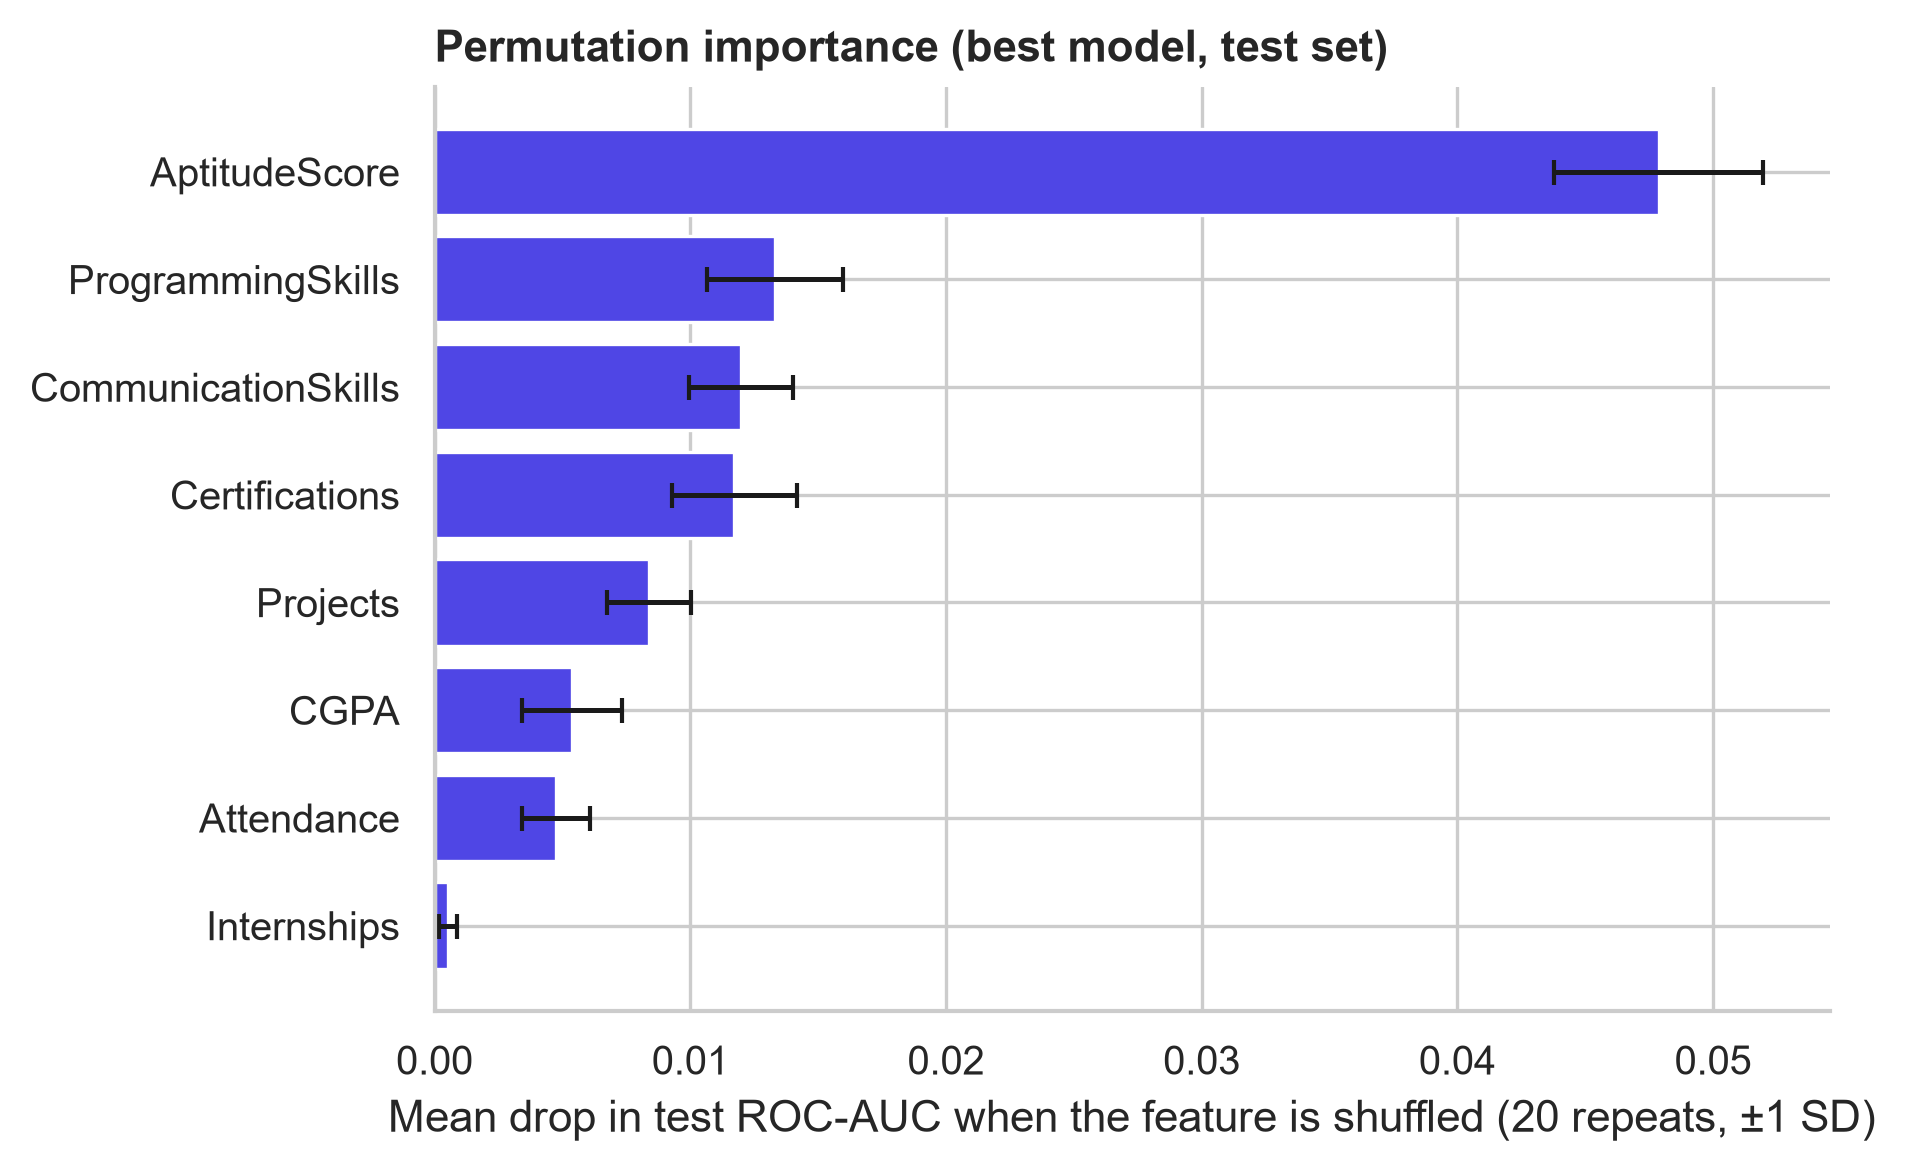
\includegraphics[width=0.49\columnwidth]{permutation_importance.png}
\caption{Logistic-regression coefficients with odds ratios (left) and permutation importance of the selected model (right).}
\label{fig:lr}
\end{figure}

\begin{figure*}[t]
\centering
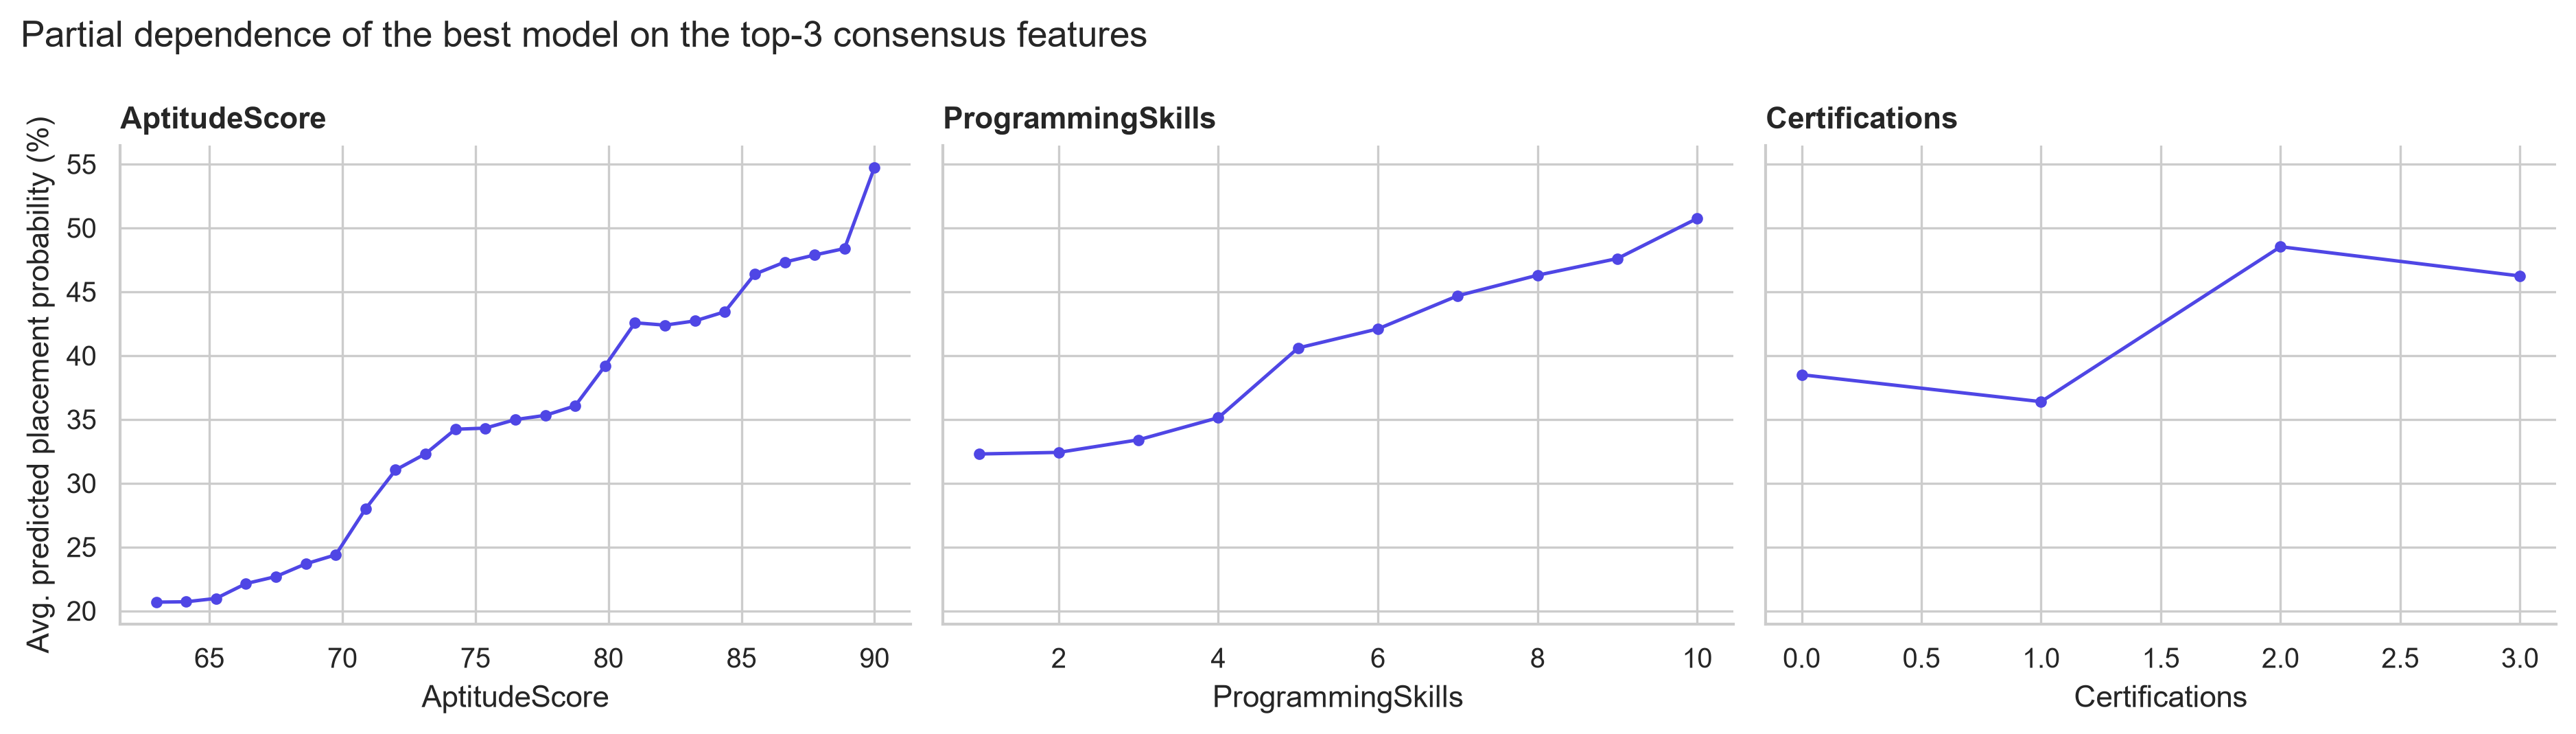
\includegraphics[width=0.85\textwidth]{pdp_top3.png}
\caption{Partial dependence of the selected model on the three most influential attributes.}
\label{fig:pdp}
\end{figure*}

\subsection{Ablation study}\label{sec:ablation}
Table~\ref{tab:abl} reports the CV ROC-AUC of the selected model type with different feature sets. Engineered
features change the score by \AblEng{} and are not used. Removing both simulated attributes changes it by
\AblNoSim{}, so the overall predictive performance does not rely on them. Adding the four extra Kaggle columns
(extracurricular activities, placement training, SSC and HSC marks) improves the score by \AblExtra{}; they
were excluded from the main model because the problem statement defines the eight core attributes, but they are
worth collecting in practice.

\begin{table}[t]
\centering
\caption{Ablation: CV ROC-AUC of \BestModel{} with different feature sets}
\label{tab:abl}
\footnotesize
\setlength{\tabcolsep}{3pt}
\begin{tabular}{lrrr}
\toprule
Feature set & \# & CV ROC-AUC & $\Delta$ \\
\midrule
(a) 8 core features & 8 & 0.8646 $\pm$ 0.0047 & +0.0000 \\
(b) core + engineered & 11 & 0.8638 $\pm$ 0.0041 & -0.0008 \\
(c) core + extra Kaggle columns & 12 & 0.8830 $\pm$ 0.0050 & +0.0185 \\
(d) core - simulated columns & 6 & 0.8564 $\pm$ 0.0055 & -0.0081 \\
\bottomrule
\end{tabular}

\end{table}

\subsection{Strengths and limitations of the models}
Table~\ref{tab:sl} summarises the qualitative trade-offs. Because the predictive performance of the five models is
nearly identical, interpretability, calibration and deployment cost become the deciding factors in practice.

\begin{table}[t]
\centering
\caption{Strengths and limitations of the models}
\label{tab:sl}
\footnotesize
\begin{tabular}{p{1.3cm}p{3.0cm}p{3.2cm}}
\toprule
Model & Strengths & Limitations \\
\midrule
LR & Transparent coefficients and odds ratios; fast & Assumes additive, monotonic log-odds effects \\
KNN & No training phase; non-parametric & Slow prediction; sensitive to scaling; no global explanation \\
SVM & Flexible non-linear boundary & Slowest to tune; probabilities need extra calibration \\
RF & Robust; little tuning needed & Large model file; biased impurity importance \\
\XGBName{} & Best CV ROC-AUC; fast; well calibrated here & More hyper-parameters; less transparent than LR \\
\bottomrule
\end{tabular}
\end{table}

\subsection{Recommendations for the placement cell}
Based on the consensus ranking and the partial dependence results: (1) prioritise aptitude training, since aptitude
score is the strongest and most consistent predictor; (2) encourage certifications and project work, which show
step-wise gains in the partial dependence plots; (3) strengthen communication-skill training; (4) use the batch-prediction page early in
the final year to identify high-risk students and use the what-if panel to agree individual, realistic goals;
and (5) record programming-skill and attendance data properly, so that their real effect can be measured instead
of simulated.

% ===========================================================================
\section{Conclusion and Future Work}\label{sec:conclusion}
This paper presented a reproducible pipeline that predicts campus placement from eight student attributes,
compared five classifiers, and identified the most influential attributes with five independent methods.
\BestModel{} was selected with a test ROC-AUC of \BestTestAUC{}, although its advantage over \SecondModel{}
\StatSig{} statistically significant. \TopOne{}, \TopTwo{} and \TopThree{} emerged as the most influential
attributes. The model is deployed in a web application that explains individual predictions and suggests
concrete improvements.

\textbf{Limitations.} Two of the eight attributes are simulated, so their influence reflects modelling
assumptions; the data-quality problems were injected rather than observed; only one public dataset was used, and
that dataset may itself be partly synthetic. The results should therefore be validated before any operational use.

\textbf{Future work.} Future work includes (i) collecting real institutional data with genuine programming
assessments and attendance records; (ii) adding attributes such as branch, backlogs and company tier; (iii) a
fairness analysis across gender and background; (iv) evaluating deep tabular models; and (v) temporal validation
on a new graduating batch.

\bibliographystyle{IEEEtran}
\bibliography{references}

\end{document}
